% Options for packages loaded elsewhere
\PassOptionsToPackage{unicode}{hyperref}
\PassOptionsToPackage{hyphens}{url}
\documentclass[
  12pt,
]{article}
\usepackage{xcolor}
\usepackage[margin=1in]{geometry}
\usepackage{amsmath,amssymb}
\setcounter{secnumdepth}{-\maxdimen} % remove section numbering
\usepackage{iftex}
\ifPDFTeX
  \usepackage[T1]{fontenc}
  \usepackage[utf8]{inputenc}
  \usepackage{textcomp} % provide euro and other symbols
\else % if luatex or xetex
  \usepackage{unicode-math} % this also loads fontspec
  \defaultfontfeatures{Scale=MatchLowercase}
  \defaultfontfeatures[\rmfamily]{Ligatures=TeX,Scale=1}
\fi
\usepackage{lmodern}
\ifPDFTeX\else
  % xetex/luatex font selection
\fi
% Use upquote if available, for straight quotes in verbatim environments
\IfFileExists{upquote.sty}{\usepackage{upquote}}{}
\IfFileExists{microtype.sty}{% use microtype if available
  \usepackage[]{microtype}
  \UseMicrotypeSet[protrusion]{basicmath} % disable protrusion for tt fonts
}{}
\makeatletter
\@ifundefined{KOMAClassName}{% if non-KOMA class
  \IfFileExists{parskip.sty}{%
    \usepackage{parskip}
  }{% else
    \setlength{\parindent}{0pt}
    \setlength{\parskip}{6pt plus 2pt minus 1pt}}
}{% if KOMA class
  \KOMAoptions{parskip=half}}
\makeatother
\usepackage{graphicx}
\makeatletter
\newsavebox\pandoc@box
\newcommand*\pandocbounded[1]{% scales image to fit in text height/width
  \sbox\pandoc@box{#1}%
  \Gscale@div\@tempa{\textheight}{\dimexpr\ht\pandoc@box+\dp\pandoc@box\relax}%
  \Gscale@div\@tempb{\linewidth}{\wd\pandoc@box}%
  \ifdim\@tempb\p@<\@tempa\p@\let\@tempa\@tempb\fi% select the smaller of both
  \ifdim\@tempa\p@<\p@\scalebox{\@tempa}{\usebox\pandoc@box}%
  \else\usebox{\pandoc@box}%
  \fi%
}
% Set default figure placement to htbp
\def\fps@figure{htbp}
\makeatother
% definitions for citeproc citations
\NewDocumentCommand\citeproctext{}{}
\NewDocumentCommand\citeproc{mm}{%
  \begingroup\def\citeproctext{#2}\cite{#1}\endgroup}
\makeatletter
 % allow citations to break across lines
 \let\@cite@ofmt\@firstofone
 % avoid brackets around text for \cite:
 \def\@biblabel#1{}
 \def\@cite#1#2{{#1\if@tempswa , #2\fi}}
\makeatother
\newlength{\cslhangindent}
\setlength{\cslhangindent}{1.5em}
\newlength{\csllabelwidth}
\setlength{\csllabelwidth}{3em}
\newenvironment{CSLReferences}[2] % #1 hanging-indent, #2 entry-spacing
 {\begin{list}{}{%
  \setlength{\itemindent}{0pt}
  \setlength{\leftmargin}{0pt}
  \setlength{\parsep}{0pt}
  % turn on hanging indent if param 1 is 1
  \ifodd #1
   \setlength{\leftmargin}{\cslhangindent}
   \setlength{\itemindent}{-1\cslhangindent}
  \fi
  % set entry spacing
  \setlength{\itemsep}{#2\baselineskip}}}
 {\end{list}}
\usepackage{calc}
\newcommand{\CSLBlock}[1]{\hfill\break\parbox[t]{\linewidth}{\strut\ignorespaces#1\strut}}
\newcommand{\CSLLeftMargin}[1]{\parbox[t]{\csllabelwidth}{\strut#1\strut}}
\newcommand{\CSLRightInline}[1]{\parbox[t]{\linewidth - \csllabelwidth}{\strut#1\strut}}
\newcommand{\CSLIndent}[1]{\hspace{\cslhangindent}#1}
\setlength{\emergencystretch}{3em} % prevent overfull lines
\providecommand{\tightlist}{%
  \setlength{\itemsep}{0pt}\setlength{\parskip}{0pt}}
\usepackage{setspace}
\doublespacing
\usepackage{lineno}
\linenumbers
\usepackage{hyperref}
\usepackage{bookmark}
\IfFileExists{xurl.sty}{\usepackage{xurl}}{} % add URL line breaks if available
\urlstyle{same}
\hypersetup{
  pdftitle={Soil properties and sediment accretion modulate methane fluxes from restored wetlands},
  pdfauthor={Samuel D Chamberlain1, Tyler Anthony1, Whendee L Silver1, Elke Eichelmann1, Kyle S Hemes1, Patricia Y Oikawa2, Cove Sturtevant3, Daphne J Szutu1, Joseph G Verfaillie1, and Dennis D Baldocchi1},
  hidelinks,
  pdfcreator={LaTeX via pandoc}}

\title{Soil properties and sediment accretion modulate methane fluxes
from restored wetlands}
\author{Samuel D Chamberlain\textsuperscript{1}, Tyler
Anthony\textsuperscript{1}, Whendee L Silver\textsuperscript{1}, Elke
Eichelmann\textsuperscript{1}, Kyle S Hemes\textsuperscript{1}, Patricia
Y Oikawa\textsuperscript{2}, Cove Sturtevant\textsuperscript{3}, Daphne
J Szutu\textsuperscript{1}, Joseph G Verfaillie\textsuperscript{1}, and
Dennis D Baldocchi\textsuperscript{1}}
\date{2026-03-20}

\begin{document}
\maketitle

\textsuperscript{1}Department of Environmental Science, Policy, and
Management, University of California, Berkeley, California, USA

\textsuperscript{2}Department of Earth and Environmental Sciences,
California State University, East Bay, Hayward, California, USA

\textsuperscript{3}National Ecological Observatory Network, Battelle,
Boulder, Colorado, USA

\textbf{Running Head}: Wetland CH\textsubscript{4} emission and soil
interactions

\textbf{Keywords}: eddy covariance, greenhouse gas balance, carbon flux,
peatland, redox, alternative electron acceptor, Sacramento-San Joaquin
Delta, information theory

\textbf{Type of Paper}: Primary research article

\newpage

\section{Abstract}\label{abstract}

Wetlands are the largest source of methane (CH\textsubscript{4})
globally, yet our understanding of how process-level controls scale to
ecosystem fluxes remains limited. It is particularly uncertain how
variable soil properties influence ecosystem CH\textsubscript{4}
emissions on annual time scales. We measured ecosystem carbon dioxide
(CO\textsubscript{2}) and CH\textsubscript{4} fluxes by eddy covariance
from two wetlands recently restored on peat and alluvium soils within
the Sacramento-San Joaquin Delta of California. Annual
CH\textsubscript{4} fluxes from the alluvium wetland were significantly
lower than the peat site for multiple years following restoration, but
these differences were not explained by variation in dominant climate
drivers or productivity across wetlands. Soil iron (Fe) concentrations
were significantly higher in alluvium soils, and alluvium
CH\textsubscript{4} fluxes were decoupled from plant processes compared
to the peat site, as expected when Fe reduction inhibits
CH\textsubscript{4} production in the rhizosphere. Soil carbon content
and CO\textsubscript{2} uptake rates did not vary across wetlands and
thus could also be ruled out as drivers of initial CH\textsubscript{4}
flux differences. Differences in wetland CH\textsubscript{4} fluxes
across soil types were transient; alluvium wetland fluxes were similar
to peat wetland fluxes three years after restoration. Changing alluvium
CH\textsubscript{4} emissions with time could not be explained by an
empirical model based on dominant CH\textsubscript{4} flux biophysical
drivers, suggesting that other factors, not measured by our eddy
covariance towers, were responsible for these changes. Recently accreted
alluvium soils were less acidic and contained more reduced Fe compared
to the pre-restoration parent soils, suggesting that CH\textsubscript{4}
emissions increased as conditions became more favorable to
methanogenesis within wetland sediments. This study suggests that
alluvium soil properties, likely Fe content, are capable of inhibiting
ecosystem-scale wetland CH\textsubscript{4} flux, but these effects
appear to be transient without continued input of alluvium to wetland
sediments.

\newpage

\section{Introduction}\label{introduction}

Wetlands play a fundamental role in regulating global climate and are
important biogeochemical hotspots, as they store \textasciitilde18\% of
Earth's soil carbon (C) (\citeproc{ref-lal_carbon_2008}{Lal, 2008}),
emit \textasciitilde30\% of global methane (CH\textsubscript{4})
emissions (\citeproc{ref-kirschke_three_2013}{Kirschke \emph{et al.},
2013}; \citeproc{ref-saunois_global_2016}{Saunois \emph{et al.}, 2016}),
while only occupying 5-8\% of the terrestrial land surface
(\citeproc{ref-mitsch_wetlands_2013}{Mitsch \emph{et al.}, 2013}). Most
wetlands are greenhouse gas (GHG) sinks over multi-century time scales
due to carbon dioxide (CO\textsubscript{2}) sequestration within anoxic
soils, though they are commonly GHG sources over shorter time scales due
to the high global warming potential of CH\textsubscript{4} they emit
(\citeproc{ref-whiting_greenhouse_2001}{Whiting \& Chanton, 2001};
\citeproc{ref-mitsch_wetlands_2013}{Mitsch \emph{et al.}, 2013};
\citeproc{ref-neubauer_moving_2015}{Neubauer \& Megonigal, 2015};
\citeproc{ref-petrescu_uncertain_2015}{Petrescu \emph{et al.}, 2015}).
Wetland C sequestration and CH\textsubscript{4} emissions are
inextricably linked, as anoxic soil conditions inhibiting ecosystem
respiration (\emph{ER}) also activates archaeal CH\textsubscript{4}
production (\citeproc{ref-whalen_biogeochemistry_2005}{Whalen, 2005};
\citeproc{ref-conrad_global_2009}{Conrad, 2009}), though recent studies
suggest significant CH\textsubscript{4} production also occurs in the
oxic zone (\citeproc{ref-angle_methanogenesis_2017}{Angle \emph{et al.},
2017}). The balance between these opposing fluxes primarily determines
wetland GHG balances (\citeproc{ref-bubier_ecological_1994}{Bubier \&
Moore, 1994}; \citeproc{ref-hendriks_full_2007}{Hendriks \emph{et al.},
2007}; \citeproc{ref-petrescu_uncertain_2015}{Petrescu \emph{et al.},
2015}), and small differences in sustained ecosystem CH\textsubscript{4}
emissions can induce large changes in wetland GHG exchange due to the
\textgreater{} 45-fold radiative forcing of CH\textsubscript{4} compared
to CO\textsubscript{2} over decadal to centennial time horizons
(\citeproc{ref-neubauer_moving_2015}{Neubauer \& Megonigal, 2015}).
Recent rises in atmospheric CH\textsubscript{4} have been attributed to
a global increase in wetland CH\textsubscript{4} fluxes
(\citeproc{ref-nisbet_rising_2016}{Nisbet \emph{et al.}, 2016}), and
wetlands are currently the most uncertain component of the global
CH\textsubscript{4} budget (\citeproc{ref-kirschke_three_2013}{Kirschke
\emph{et al.}, 2013}). A key driver of this uncertainty is a lack of
ecosystem-scale flux measurements to better constrain models and improve
our understanding of how process-level controls scale to whole ecosystem
CH\textsubscript{4} emissions
(\citeproc{ref-bridgham_methane_2013}{Bridgham \emph{et al.}, 2013};
\citeproc{ref-saunois_global_2016}{Saunois \emph{et al.}, 2016}).

Methane fluxes from wetlands are governed by many interacting
biophysical drivers including temperature, C inputs, alternative
electron acceptor pools, and water table depth
(\citeproc{ref-bridgham_methane_2013}{Bridgham \emph{et al.}, 2013}). It
is uncertain how these governing factors interact and scale to whole
ecosystem fluxes due to sparse global coverage of ecosystem-scale eddy
covariance flux sites (\citeproc{ref-petrescu_uncertain_2015}{Petrescu
\emph{et al.}, 2015}), where current measurement campaigns may
under-sample relevant environmental gradients. Chamber flux syntheses
have demonstrated that water table depth, temperature, vegetation,
disturbance, and wetland type are important modulators of wetland
CH\textsubscript{4} flux
(\citeproc{ref-turetsky_synthesis_2014}{Turetsky \emph{et al.}, 2014}).
A similar understanding of the controls on CH\textsubscript{4} fluxes is
emerging from eddy covariance studies, where temperature
(\citeproc{ref-rinne_annual_2007}{Rinne \emph{et al.}, 2007};
\citeproc{ref-wille_methane_2008}{Wille \emph{et al.}, 2008};
\citeproc{ref-hendriks_multi-technique_2010}{Hendriks \emph{et al.},
2010}; \citeproc{ref-olson_interannual_2013}{Olson \emph{et al.}, 2013};
\citeproc{ref-chu_net_2014}{Chu \emph{et al.}, 2014}), recent C inputs
(\citeproc{ref-hatala_gross_2012}{Hatala \emph{et al.}, 2012a};
\citeproc{ref-morin_environmental_2014}{Morin \emph{et al.}, 2014}),
wetland structure (\citeproc{ref-matthes_parsing_2014}{Matthes \emph{et
al.}, 2014}; \citeproc{ref-mcnicol_effects_2017}{McNicol \emph{et al.},
2017}), vegetation cover (\citeproc{ref-morin_combining_2017}{Morin
\emph{et al.}, 2017};
\citeproc{ref-rey-sanchez_determining_2017}{Rey-Sanchez \emph{et al.},
2017}) and water table depth (\citeproc{ref-hendriks_full_2007}{Hendriks
\emph{et al.}, 2007},
\citeproc{ref-hendriks_multi-technique_2010}{2010};
\citeproc{ref-brown_evidence_2014}{Brown \emph{et al.}, 2014};
\citeproc{ref-chamberlain_underlying_2015}{Chamberlain \emph{et al.},
2015}, \citeproc{ref-chamberlain_influence_2016}{2016},
\citeproc{ref-chamberlain_impact_2017}{2017a};
\citeproc{ref-goodrich_overriding_2015}{Goodrich \emph{et al.}, 2015};
\citeproc{ref-sturtevant_identifying_2016}{Sturtevant \emph{et al.},
2016}) have been identified as dominant controls across many wetland
ecosystems. Combined chamber and eddy covariance studies have further
improved our understanding of how drivers of small-scale flux variation
scale to ecosystem fluxes
(\citeproc{ref-forbrich_cross-evaluation_2011}{Forbrich \emph{et al.},
2011}; \citeproc{ref-morin_combining_2017}{Morin \emph{et al.}, 2017};
\citeproc{ref-rey-sanchez_determining_2017}{Rey-Sanchez \emph{et al.},
2017}).

Small-scale field and laboratory studies have also demonstrated the
influence of soil C content (\citeproc{ref-levy_methane_2012}{Levy
\emph{et al.}, 2012}; \citeproc{ref-bridgham_methane_2013}{Bridgham
\emph{et al.}, 2013}; \citeproc{ref-ye_soil_2016}{Ye \emph{et al.},
2016}) and alternative electron acceptor pools, such as sulfate and
ferric iron, on wetland CH\textsubscript{4} fluxes
(\citeproc{ref-laanbroek_methane_2010}{Laanbroek, 2010};
\citeproc{ref-poffenbarger_salinity_2011}{Poffenbarger \emph{et al.},
2011}; \citeproc{ref-bridgham_methane_2013}{Bridgham \emph{et al.},
2013}; \citeproc{ref-miller_methane_2015}{Miller \emph{et al.}, 2015}).
Recently, Holm \emph{et al.} (\citeproc{ref-holm_ecosystem_2016}{2016})
and Krauss \emph{et al.} (\citeproc{ref-krauss_component_2016}{2016})
used eddy covariance to observe reductions in coastal wetland
CH\textsubscript{4} fluxes with increasing salinity, speculatively due
to sulfate redox inhibition of methanogenesis
(\citeproc{ref-poffenbarger_salinity_2011}{Poffenbarger \emph{et al.},
2011}), demonstrating how redox conditions can modulate annual
CH\textsubscript{4} emissions. Iron (Fe) minerals can also inhibit
CH\textsubscript{4} production and emissions
(\citeproc{ref-laanbroek_methane_2010}{Laanbroek, 2010}), as observed in
many laboratory and field studies
(\citeproc{ref-jackel_suppression_2000}{Jäckel \& Schnell, 2000};
\citeproc{ref-neubauer_seasonal_2005}{Neubauer \emph{et al.}, 2005};
\citeproc{ref-teh_suppression_2008}{Teh \emph{et al.}, 2008};
\citeproc{ref-ali_silicate_2009}{Ali \emph{et al.}, 2009};
\citeproc{ref-zhou_methanogenesis_2014}{Zhou \emph{et al.}, 2014}),
though Fe inhibition to long-term ecosystem fluxes has not been
documented by eddy covariance. Understanding the interactions between
soil properties, such as Fe content, and CH\textsubscript{4} emissions
may be particularly important to upscaling and modeling fluxes across
complex, heterogeneous landscapes, such as river deltas or the tropics,
the largest source of the global wetland CH\textsubscript{4} emissions
(\citeproc{ref-kirschke_three_2013}{Kirschke \emph{et al.}, 2013}),
where high Fe concentrations influence rates of organic matter
decomposition and CH\textsubscript{4} production
(\citeproc{ref-teh_suppression_2008}{Teh \emph{et al.}, 2008};
\citeproc{ref-dubinsky_tropical_2010}{Dubinsky \emph{et al.}, 2010};
\citeproc{ref-hall_iron_2013}{Hall \& Silver, 2013}).

Wetland restoration and management programs have increasingly been
proposed and implemented to mitigate climate change
(\citeproc{ref-mitsch_creating_1998}{Mitsch \emph{et al.}, 1998};
\citeproc{ref-mitsch_wetlands_2013}{Mitsch \emph{et al.}, 2013}), and
restoration strategies that minimize CH\textsubscript{4} emissions and
maximize CO\textsubscript{2} uptake will provide the optimum climate
benefit. These programs are particularly appealing in coastal ecosystems
where CO\textsubscript{2} sequestration rates are high and
CH\textsubscript{4} flux rates are low
(\citeproc{ref-poffenbarger_salinity_2011}{Poffenbarger \emph{et al.},
2011}; \citeproc{ref-conservation_international_blue}{Conservation
International, 2017}), and in drained peatlands where large
CO\textsubscript{2} emissions from oxidizing peat can be reduced by
re-flooding the landscape (\citeproc{ref-hatala_greenhouse_2012}{Hatala
\emph{et al.}, 2012b}; \citeproc{ref-knox_agricultural_2015}{Knox
\emph{et al.}, 2015}; \citeproc{ref-wilson_multiyear_2016}{Wilson
\emph{et al.}, 2016}). A thorough understanding of CH\textsubscript{4}
flux drivers is essential to these programs because the magnitude of
CH\textsubscript{4} emissions may determine if restored wetlands are a
GHG source or sink (\citeproc{ref-knox_agricultural_2015}{Knox \emph{et
al.}, 2015}). These emissions could affect funding of wetland
restoration programs if financed through C markets alone
(\citeproc{ref-oikawa_evaluation_2017}{Oikawa \emph{et al.}, 2017a}),
though wetlands provide a number of relevant ecosystem services, such as
nutrient retention, protection from storms and sea-level rise, and
habitat preservation for wildlife
(\citeproc{ref-hansson_conflicting_2005}{Hansson \emph{et al.}, 2005};
\citeproc{ref-zedler2005wetland}{Zedler \& Kercher, 2005};
\citeproc{ref-swain_trade-offs_2013}{Swain \emph{et al.}, 2013}).

The Sacramento-San Joaquin Delta region of California (hereafter
referred to as the Delta) is an area where financing of wetland
restoration through California's Cap and Trade program is being
considered. The Delta is comprised of a network of artificially drained
islands reclaimed for agriculture, where the water table is maintained
below sea level by active pumping and levees surrounding each island.
Drainage began in the 1850's to facilitate agricultural development, and
exposure of the highly organic soils has led to substantial land surface
subsidence (\citeproc{ref-deverel_historic_2010}{Deverel \& Leighton,
2010}) and CO\textsubscript{2} emissions
(\citeproc{ref-hatala_greenhouse_2012}{Hatala \emph{et al.}, 2012b};
\citeproc{ref-knox_agricultural_2015}{Knox \emph{et al.}, 2015}), and
wetland restoration efforts aim to accrete new sediments and reduce GHG
emissions (\citeproc{ref-miller_subsidence_2008}{Miller \emph{et al.},
2008}; \citeproc{ref-miller_carbon_2011}{Miller, 2011};
\citeproc{ref-hatala_greenhouse_2012}{Hatala \emph{et al.}, 2012b}).
Prior to drainage, this region was a 2990 km\textsuperscript{2} tidal
marsh where soils varied substantially across space due to fluvial
deposition from major rivers that carried mineral alluvium from the
Sierra Nevada mountain range to the Delta marshes
(\citeproc{ref-atwater1979history}{Atwater \emph{et al.}, 1979};
\citeproc{ref-atwater1980tidal}{Atwater \& Belknap, 1980}). These
differences in pre-drainage wetland geomorphology give rise to a
contemporary agricultural landscape where large changes in soil C and
mineral content occur over small spatial scales
(\citeproc{ref-soilsurvey}{Soil Survey Staff, 2017}), but how this
edaphic variation influences current GHG fluxes from restored wetlands
is unknown. Understanding the importance of these soil legacy effects is
highly desirable, as it would allow for more informed wetland
restoration strategies where sites could be chosen to minimize GHG
emissions.

The objectives of this study were to (1) determine how soil properties
and wetland GHG fluxes varied across wetlands restored on peat versus
alluvium soils, (2) identify how relationships between biophysical
drivers and CH\textsubscript{4} fluxes varied across wetland types, and
(3) determine the most likely drivers (climate v. edaphic) of observed
flux differences. To meet these objectives, we measured ecosystem-scale
CH\textsubscript{4} and CO\textsubscript{2} fluxes by eddy covariance
from two recently restored wetlands, where one wetland was restored on
peat soils while the other was restored on alluvium soils, and measured
multiple soil properties within the tower footprints to identify
potential edaphic drivers of observed flux differences. Soil properties
were measured across two horizons as a proxy for time, and this depth
for time assumption is valid because vertical accretion of new sediments
in Sacramento-San Joaquin Delta wetlands has been documented using both
feldspar marker (\citeproc{ref-miller_subsidence_2008}{Miller \emph{et
al.}, 2008}) and radiocarbon dating methods
(\citeproc{ref-drexler_peat_2009}{Drexler \emph{et al.}, 2009};
\citeproc{ref-drexler_peat_2011}{Drexler, 2011}). We then used a
combination of wavelet analysis and information theory to identify time
scale-emergent biophysical drivers of wetland CH\textsubscript{4} fluxes
and how they varied across the wetlands. Once differences were
established, we used an empirical biophysical CH\textsubscript{4} flux
model trained on an independent mature wetland to determine whether
observed differences could be explained by common, non-edaphic
biophysical drivers alone. These tower sites are ideal for identifying
edaphic controls, as all wetlands sites have a similarly managed
hydroperiod, are within 13 km of one another, experience the same
climate, and have similar plant community compositions.

\section{Materials and Methods}\label{materials-and-methods}

\subsection{Site Description}\label{site-description}

We measured wetland ecosystem CH\textsubscript{4} and
CO\textsubscript{2} fluxes using a network of eddy covariance towers in
the Sacramento-San Joaquin Delta region of California, USA. The Delta is
located within a Mediterranean climate that experiences hot, dry summers
and cooler, rainy winters. The mean annual temperature is 15.1
\(^\circ\)C (1998-2015 average), and the region receives 326 mm of
rainfall annually (\citeproc{ref-knox_biophysical_2016}{Knox \emph{et
al.}, 2016}). All measurement sites were located on Sherman and
Twitchell Islands in the northwest Delta. These islands are a mosaic of
alluvium mollisols and highly organic peat histosols
(\citeproc{ref-soilsurvey}{Soil Survey Staff, 2017}). Alluvium marsh
mollisols frequently developed adjacent to peat histosols that were
spatially segregated from the main river channels
(\citeproc{ref-atwater1979history}{Atwater \emph{et al.}, 1979};
\citeproc{ref-atwater1980tidal}{Atwater \& Belknap, 1980}). Alluvium
soils formed via fluvial deposition from major rivers and are most
common on islands adjacent to the Sacramento River compared to the
central and eastern Delta region where fluvial deposition was less
pronounced (\citeproc{ref-deverel_historic_2010}{Deverel \& Leighton,
2010}). These alluvium soils tend to be high in Fe content, as the
Sacramento River drains the northern Sierra Nevada range where Fe
concentrations are particularly high compared to the central or south
Sierra Nevada (\citeproc{ref-graham_soil_2010}{Graham \& O'Geen, 2010}).
In contrast, peat histosols formed densely organic soils in areas less
disturbed by fluvial input (\citeproc{ref-deverel_historic_2010}{Deverel
\& Leighton, 2010}). The dominant mollisol series on these islands are
Gazwell and Scribner (Fig. 1), both of which are formed in mixed
alluvium, belong to the soil class Cumulic Endoaquolls, and are only
found on Delta islands within the Sacramento River drainage
(\citeproc{ref-soilsurvey}{Soil Survey Staff, 2017}). Rindge is the
major histosol series found on both islands (Fig. 1) and is widely
distributed across the Delta region. Rindge soils belong to the Typic
Haplosaprists class, and are characterized by deep, poorly drained marsh
soils formed from decomposed plant organic matter
(\citeproc{ref-soilsurvey}{Soil Survey Staff, 2017}).

Fluxes were measured from the time of initial restoration at two sites,
where one wetland, hereafter referred to as the `peat' site (Ameriflux
site Us-Myb; N 38.0498, W 121.7650), was restored in 2010 from a pasture
on peat Rindge soils (Fig. 1a). The other recently restored site,
hereafter referred to as the `alluvium' site (Ameriflux site US-Tw4; N
38.10275, W 121.64125), was restored in 2014 from a corn field on
alluvium Scribner soils (Fig. 1b). We have also measured fluxes since
2013 from an older, mature wetland, hereafter referred to as the
`mature' site (Ameriflux site Us-Tw1; N 38.1074, W 121.6469), that was
restored in 1999 on peat Rindge soils (Fig. 1b). A detailed description
of tower instrumentation can be found in the Supplemental Materials. All
sites are vegetated predominantly by cattails (\emph{Typha} spp.), with
few tules (\emph{Schoenoplectus acutus}), and are actively managed to
remain inundated year-round. Peat and alluvium sites were constructed to
have heterogeneous bathymetry, providing channels of open water and
areas of closed vegetation. The mature site is entirely closed
vegetation and the ground surface is saturated plant detritus, whereas
the recently restored peat and alluvium sites have standing water under
the plant canopy. Given the large differences age and stand structure
between the mature wetland and other sites, most comparisons made in
this study are between the recently restored peat and alluvium sites
that have similar bathymetry, stand structure, and measurement coverage
across early successional periods. For a more detailed description of
the peat and mature sites see Miller
(\citeproc{ref-miller_carbon_2011}{2011}), Matthes \emph{et al.}
(\citeproc{ref-matthes_parsing_2014}{2014}), and Knox \emph{et al.}
(\citeproc{ref-knox_agricultural_2015}{2015}).

Flux corrections and quality control were applied as described in detail
in Knox \emph{et al.} (\citeproc{ref-knox_agricultural_2015}{2015}) and
Chamberlain \emph{et al.}
(\citeproc{ref-chamberlain_evaluation_2017}{2017b}), and included
high-frequency data despiking, 2-D coordinate rotations, density
corrections, and site-specific friction velocity (\emph{u\(^\ast\)})
filtering. At the mature site, we reject fluxes from wind directions
290\(^\circ\)-240\(^\circ\) because fluxes from these directions were
from other wetland types; however, we did not apply wind direction
filtering to the other sites where flux footprints were more
homogeneous. Footprints at all sites were calculated using a
two-dimensional analytical model
(\citeproc{ref-hsieh_approximate_2000}{Hsieh \emph{et al.}, 2000};
\citeproc{ref-detto_soil_2006}{Detto \emph{et al.}, 2006}).

We gap filled missing fluxes using artificial neural networks (ANNs), as
described in detail in Knox \emph{et al.}
(\citeproc{ref-knox_agricultural_2015}{2015}). Briefly, we used
single-layer, feed-forward ANNs with meteorological variables as inputs.
Flux data without missing values were split into training, validation,
and test sets (1/3 split), and we trained multiple ANN architectures
with varying nodes per single hidden layer, keeping the simplest
architecture where a more complex architecture led to a less than 5\%
reduction in root mean squared error. This process (including resampling
training, validation, and test data) was repeated 20 times, and the
median of the 20 ANN predictions was used to fill missing fluxes and the
variance was used to estimate gap filling uncertainty. Separate ANNs
were trained for daytime and nighttime CO\textsubscript{2} fluxes, and
the nighttime CO\textsubscript{2} flux ANN was used to model \emph{ER}
at all times. Gross ecosystem photosynthesis (\emph{GEP}) was then
estimated as the difference between the gap-filled CO\textsubscript{2}
flux and modeled \emph{ER} (\citeproc{ref-baldocchi_does_2015}{Baldocchi
\emph{et al.}, 2015}). Our partitioning method performs well against
independent verification methods in agricultural systems
(\citeproc{ref-oikawa_revisiting_2017}{Oikawa \emph{et al.}, 2017b}).

\begin{figure}
\centering
\pandocbounded{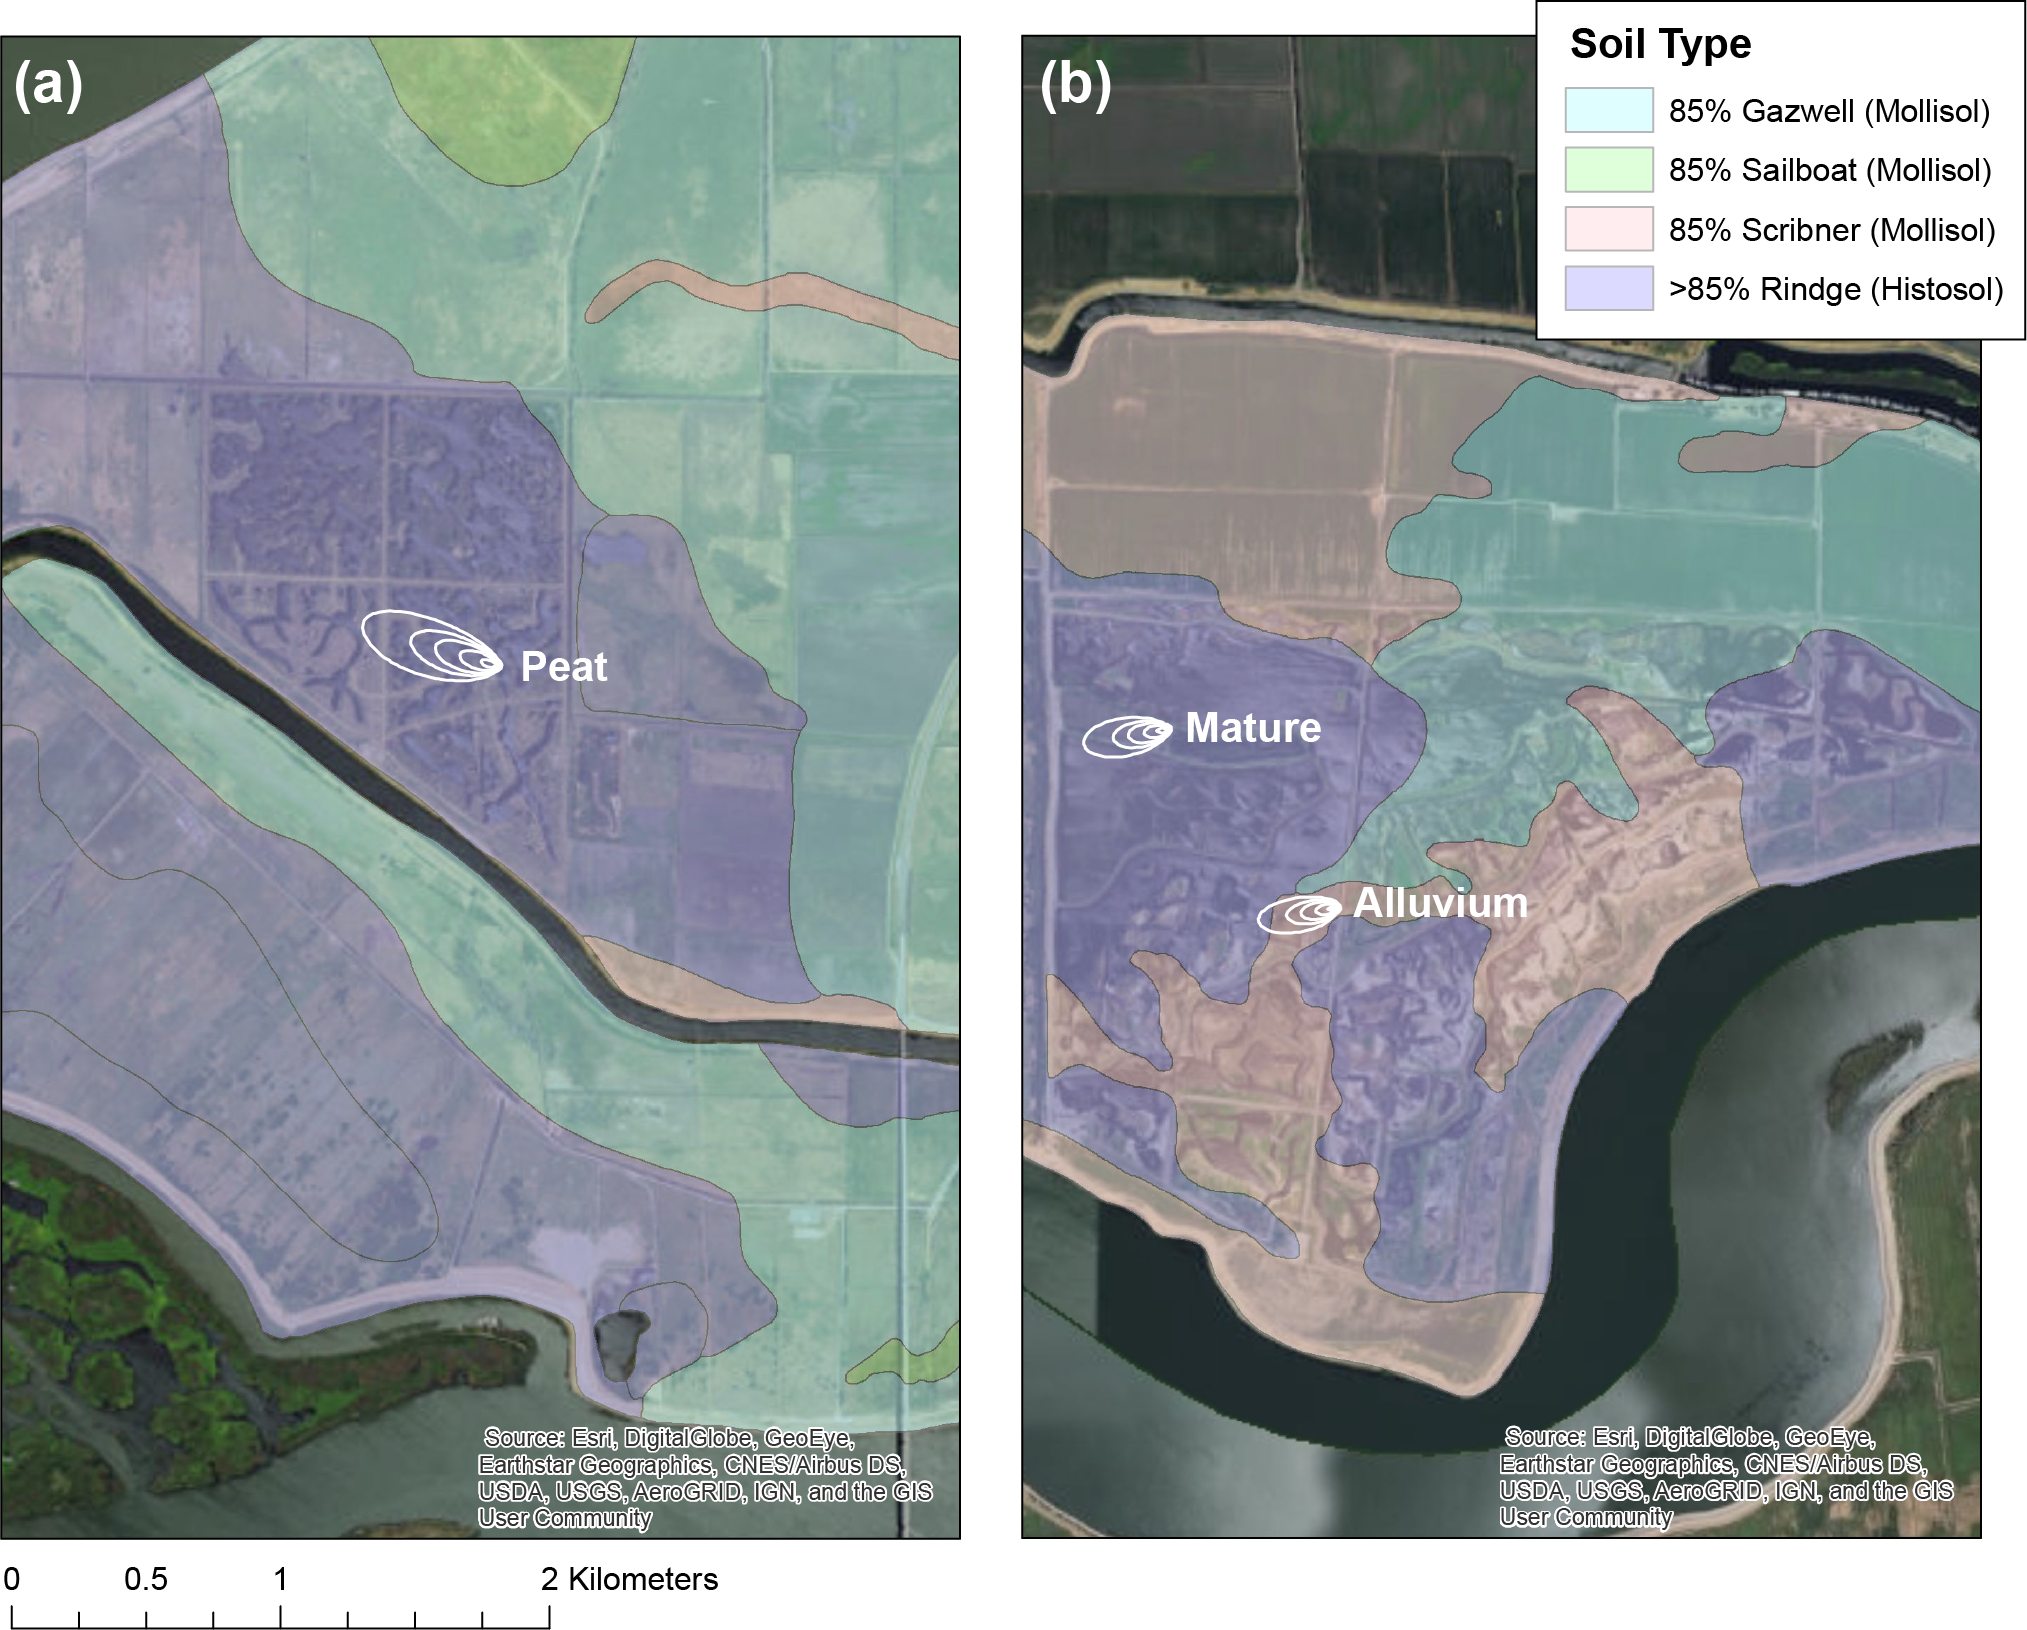
\includegraphics[keepaspectratio]{fig1.png}}
\caption{Soil type and tower flux footprints for (a) Sherman and (b)
Twitchell Islands in the Sacramento-San Joaquin Delta of California.
Tower footprints include wetland area only, and footprint rings, from
largest to smallest, correspond to the 90, 85, 80, 70, and 50\%
cumulative flux footprints at each site. Tower footprints were
calculated using a two-dimensional analytical model described in Detto
\emph{et al.} (\citeproc{ref-detto_soil_2006}{2006}). Site names are
given next to their respective footprint.}
\end{figure}

\subsection{Soil Analyses}\label{soil-analyses}

We measured soil C, N, and Fe content at the three wetland sites in the
recently accreted wetland O horizon, hereafter referred to as the
accreted horizon, and the underlying pre-restoration parent soils,
hereafter referred to as the parent horizon. Fifteen samples of both
accreted and parent horizon soils were collected at each site across
three transects, with each sampling location at least 3 m apart. The
transects were within each tower's flux footprint, all samples were
collected from fully inundated locations, and the accreted sample was
collected directly above the underlying parent soil sample. At the peat
and alluvium sites (both \textless{} 8 years old), the differentiation
between these horizons was clear, as the recently accreted horizon was
loose, mucky, and heavily comprised of poorly-decomposed plant matter,
whereas the underlying parent horizon was compacted agricultural soil.
At these sites, we collected the accreted horizon by hand (grab samples)
and the top 15 cm of parent horizon using a sediment core. Our sampling
strategy was different at the mature site because more than 0.5 m of O
horizon had accumulated since initial restoration. Here, the accreted
horizon reached the water surface, and we collected the top 2 cm of this
horizon to represent the most recently accreted peat. We then bore holes
through the 0.5-0.7 m saturated peat layer to collect the underlying
parent soil horizon. Differentiation between these layers was also
clear, as the top 0.5-0.7 m was comprised of poorly-decomposed plant
matter and the underlying horizon was a silty clay loam. These
observations are consistent with previously measured accretion rates and
peat depths (\citeproc{ref-miller_subsidence_2008}{Miller \emph{et al.},
2008}).

All soil samples were immediately bagged, and sub-samples were extracted
in the field with both 0.5 M HCl and 0.2 M sodium citrate/0.05 M sodium
ascorbate solutions to measure HCl-extractable Fe
(Fe\textsuperscript{2+} and Fe\textsuperscript{3+}) and poorly
crystalline Fe oxide pools, respectively. The HCl extraction solubilizes
reactive Fe\textsuperscript{3+} minerals and absorbed/solid
Fe\textsuperscript{2+}, and is used to quantify oxidized
(Fe\textsuperscript{3+}) and reduced (Fe\textsuperscript{2+}) Fe pools.
The low pH of HCl prevents any Fe\textsuperscript{2+} oxidation after
the samples are collected (\citeproc{ref-hall_reducing_2015}{Hall \&
Silver, 2015}). Roughly 3 g of sample (dry mass equivalent) were
immediately placed into preweighed bottles with the HCl solution, and
once back in the lab, samples were reweighed, vortexed, shaken for 1
hour, and centrifuged for 10 minutes at 1000 rcf. Concentrations of
Fe\textsuperscript{2+} and Fe\textsuperscript{3+} were measured
colorimetrically using the ferrozine assay
(\citeproc{ref-viollier_ferrozine_2000}{Viollier \emph{et al.}, 2000}).
Citrate-ascorbate extractions were used to quantify poorly crystalline
Fe oxides that are reducible by soil microbes
(\citeproc{ref-hyacinthe_reactive_2006}{Hyacinthe \emph{et al.}, 2006}).
Roughly 1.5 g of sample (dry mass equivalent) were immediately placed
into preweighed bottles of the citrate-ascorbate solution, and in the
lab, samples were reweighed, vortexed, shaken for 16 hours, and then
centrifuged for 20 minutes at 1000 rcf. Poorly crystalline Fe
concentrations were quantified using an inductively coupled plasma
optical emission spectrometer (ICP-OES; Perkin Elmer Optima 5300 DV,
Waltham, Massachusetts, USA). We then air-dried soil samples at room
temperature for analysis of C and N concentrations. Dried subsamples
were sieved to 2 mm and all major visible roots were removed by hand.
These samples were then ground to a fine powder and analyzed in
duplicate for total C and N using an elemental analyzer (CE Elantech,
Lakewood, New Jersey, USA).

\subsection{Wavelet-Information Theory
Analysis}\label{wavelet-information-theory-analysis}

We used a combination of wavelet time series decomposition and
information theory to (1) isolate major time scales of variation within
the continuous CH\textsubscript{4} flux time series, and (2) identify
scale-emergent interactions between CH\textsubscript{4} fluxes and a
number of biophysical drivers. This technique allowed us to isolate
CH\textsubscript{4} flux controls operating at hourly, diel, and
multiday timescales, and has been previously used to identify
scale-emergent controls of CH\textsubscript{4} flux at the peat and
mature wetlands (\citeproc{ref-sturtevant_identifying_2016}{Sturtevant
\emph{et al.}, 2016}). Relative mutual information
(\emph{I\textsuperscript{R}}), an information theory metric, was used to
identify relationships between variables. Mutual information is derived
from Shannon entropy (\emph{H}), a measure of uncertainty
(\citeproc{ref-shannon1998mathematical}{Shannon \& Weaver, 1998}), and
\emph{I\textsuperscript{R}} quantifies the amount of information shared
between two variables. Mutual information and other information theory
metrics, such as transfer entropy, are particularly useful for
identifying relationships in complex systems because they do not assume
linearity or other functional relationships and are capable of
identifying asynchronous relationships
(\citeproc{ref-ruddell_applying_2013}{Ruddell \emph{et al.}, 2013}). All
wavelet decomposition and entropy calculations were conducted using the
ProcessNetwork Software
(\url{http://www.mathworks.com/matlabcentral/fileexchange/41515-processnetwork-processnetwork-software}),
and a more detailed description of the approach can be found in the
Supplemental Materials and Sturtevant \emph{et al.}
(\citeproc{ref-sturtevant_identifying_2016}{2016}).

\subsection{Statistical Analyses and Data
Processing}\label{statistical-analyses-and-data-processing}

All additional data processing, statistical analysis, and visualization
was conducted in R 3.4.1 (\citeproc{ref-r_citation}{R Core Team, 2017})
using the `tidyverse' (\citeproc{ref-tidyverse}{Wickham, 2017}), `zoo'
(\citeproc{ref-zoo}{Zeileis \& Grothendieck, 2005}), `gridExtra'
(\citeproc{ref-gridExtra}{Auguie, 2016}), `ggpubr'
(\citeproc{ref-ggpubr}{Kassambara, 2017}), `lubridate'
(\citeproc{ref-lubridate}{Grolemund \& Wickham, 2011}), and `scales'
(\citeproc{ref-scales}{Wickham, 2016}) packages. We used parametric
statistics, such as ANOVA, Welch's t-tests, and Tukey's HSD, to assess
differences in soil properties across/within sites because properties
were normally distributed within soil horizons at each site. Annual GHG
budgets were calculated using the 45x 100-year sustained-flux global
warming potential for CH\textsubscript{4} presented in Neubauer \&
Megonigal (\citeproc{ref-neubauer_moving_2015}{2015}).

We also analyzed the residuals of a generalized linear model (GAM) fit
to daily CH\textsubscript{4} fluxes at the mature wetland (2014-2017)
using nine common biophysical drivers (described in Results) to assess
whether changes in alluvium CH\textsubscript{4} fluxes with time could
be explained by common, non-edaphic drivers of stable state wetland
CH\textsubscript{4} flux. The GAM was fit using the `caret'
(\citeproc{ref-caret}{Jed Wing \emph{et al.}, 2017}) and `mgcv'
(\citeproc{ref-mgcv}{Wood, 2017}) R packages, where smoothing parameters
were chosen by generalized cross-validation and inclusion of feature
selection was chosen by using the model formulation with the lowest root
mean squared error following ten-fold cross-validation. The trained GAM
was then used to predict CH\textsubscript{4} fluxes at the peat and
alluvium wetlands.Prior to model training and prediction, missing values
in the biophysical driver data were imputed using k-nearest neighbors,
where all values were centered and scaled. This manuscript is
reproducible via R Markdown, and its code can be found at
\url{https://github.com/samdchamberlain/wetlandcomparison}. The
wavelet-information theory analysis was conducted using MATLAB and is
not directly reproducible in R; however, MATLAB source code
(\url{https://github.com/samdchamberlain/ProcessNetwork_Software}) is
available online with this manuscript.

\section{Results}\label{results}

\begin{verbatim}
#> `summarise()` has regrouped the output.
#> `summarise()` has regrouped the output.
#> `summarise()` has regrouped the output.
#> `summarise()` has regrouped the output.
#> `summarise()` has regrouped the output.
#> `summarise()` has regrouped the output.
#> i Summaries were computed grouped by dday and site.
#> i Output is grouped by dday.
#> i Use `summarise(.groups = "drop_last")` to silence this message.
#> i Use `summarise(.by = c(dday, site))` for per-operation grouping (`?dplyr::dplyr_by`) instead.
\end{verbatim}

\subsection{Soil Properties}\label{soil-properties}

Extractable Fe concentrations were significantly higher in recently
accreted and parent alluvium soil horizons compared to those at the peat
wetland (Tukey's HSD, \emph{P} \textless{} 0.001) (Fig. 2a). Extractable
Fe concentrations trended lower in the accreted compared to parent
horizon at both wetlands, but these differences were not significant
(Fig. 2a). Appreciable quantities of Fe\textsuperscript{3+} were present
in all site horizons, where 28.02\% and 33.87\% of extractable Fe was in
Fe\textsuperscript{3+} form at the alluvium and peat sites,
respectively. Most Fe was in the reduced Fe\textsuperscript{2+} form
across both sites, and statistical trends in Fe\textsuperscript{2+}
concentrations were similar to total extractable Fe (Fig. 2b). While
total extractable Fe concentrations did not vary between horizons at the
alluvium site, Fe\textsuperscript{2+} concentrations were significantly
higher in the accreted horizon compared to its underlying parent soil
(Welch's t, \emph{P} \textless{} 0.001).

Poorly crystalline Fe oxide concentrations were roughly two orders of
magnitude lower than HCl-extractable Fe concentrations across both sites
(Fig. 2c), and trends were similar to HCl-extractable Fe. Poorly
crystalline Fe concentrations were significantly higher at the alluvium
site in both soil horizons (Tukey's HSD, \emph{P} \textless{} 0.0001),
and did not vary between horizons at either wetland (Fig. 2c). Mean
poorly crystalline Fe concentrations were roughly an order of magnitude
higher in alluvium soils (0.32 \(\pm\) 0.09 mg Fe g\textsuperscript{-1}
soil; \emph{n} = 30) compared to peat soils (0.04 \(\pm\) 0.04 mg Fe
g\textsuperscript{-1} soil; \emph{n} = 30).

Soil pH also varied across the wetlands (ANOVA, \emph{P} \textless{}
0.05), where alluvium soils were acidic (5.62 \(\pm\) 0.48; \emph{n} =
30) and peat soils were near-neutral (6.99 \(\pm\) 0.33; \emph{n} = 28)
(Fig. 2d). pH did not vary by depth at the peat wetland; however, the
parent horizon was significantly more acidic at the alluvium wetland
(Welch's t, \emph{P} \textless{} 0.0001) (Fig. 2d).

Parent horizon C concentrations did not vary between the peat and
alluvium wetlands (Tukey's HSD, \emph{P} = 0.50) (Fig. 2e). Significant
differences in C concentrations were observed in the accreted horizon
(Tukey's HSD, \emph{P} \textless{} 0.0001), where C concentrations were
higher at the peat site (15.64 \(\pm\) 5.23\%; \emph{n} = 14) than the
alluvium site (10.18 \(\pm\) 1.49\%; \emph{n} = 15). Soil C
concentrations were higher in the recently accreted horizon at the peat
site (Welch's t, \emph{P} \textless{} 0.001), but no differences in C
concentration were observed between horizons at the alluvium wetland
(Fig. 2e). Similar patterns were observed for soil N concentrations
across sites; however, parent horizon N concentrations were
significantly lower at the alluvium compared to peat site (Tukey's HSD,
\emph{P} = 0.01) (Fig. 2f).

\begin{figure}
\centering
\pandocbounded{\includegraphics[keepaspectratio]{manuscript_files/figure-latex/fig2-1.pdf}}
\caption{Soil (a) HCl-extractable Fe, (b) ferrous iron
(Fe\textsuperscript{2+}), (c) poorly crystalline Fe oxides
(Fe\textsubscript{ca}), (d) pH, (e) C concentration (\%), and (f) N
concentration (\%) in accreted and parent horizons across the peat and
alluvium wetlands (\emph{n} \(\geq\) 12 per depth). Solid horizontal
lines are medians, boxes are the interquartile range, whiskers are the
95\% confidence interval, and points denote measured outliers.
Significance levels are shown for pairwise comparisons between soil
horizons at each site (Welch's t-test), where ns denotes no significant
differences and increasing asterisks denotes significance levels from
\emph{P} \textless{} 0.05, 0.01, 0.001, to 0.0001.}
\end{figure}

\subsection{Post-restoration Flux
Trajectories}\label{post-restoration-flux-trajectories}

Methane flux trajectories from the peat and alluvium wetlands were quite
different following initial restoration, where flux magnitudes were
considerably lower from the alluvium site for the first three years
following restoration and later converged with the peat site (Fig. 3a).
Across both sites, in the first year wetlands were open water and
non-vegetated, leading to low CH\textsubscript{4} flux and \emph{NEE}
compared to following years (Fig. 3), and by the second year both sites
were fully vegetated. Alluvium wetland fluxes increased with each year,
whereas CH\textsubscript{4} fluxes from the peat wetland peaked during
the second year and decreased with subsequent years (Figs. 3a).
Differences in daily fluxes across wetlands were largest during the
second year when alluvium wetland fluxes were increasing and peat
wetland emissions were peaking (Fig. 3a). Annual CH\textsubscript{4}
budgets for the peat site were over two times larger than the alluvium
site during the first and second year. First year budgets were 16.35
\(\pm\) 2.2 and 35.63 \(\pm\) 4.16 g CH\textsubscript{4}-C
m\textsuperscript{-2} yr\textsuperscript{-1} (mean \(\pm\) 95\% CI) for
the alluvium and peat wetland, respectively, and second year budgets
were 27.77 \(\pm\) 2.51 and 63.37 \(\pm\) 3.56 g CH\textsubscript{4}-C
m\textsuperscript{-2} yr\textsuperscript{-1} for the alluvium and peat
wetland, respectively. This gap began to close during year three, and
fluxes were similar across sites by year four (Fig. 3a), when annual
fluxes were 49.16 \(\pm\) 3.71 and 57.17 \(\pm\) 3.51 g
CH\textsubscript{4}-C m\textsuperscript{-2} yr\textsuperscript{-1} from
the alluvium and peat wetland, respectively.

Differences in \emph{NEE} were less notable across the two recently
restored wetlands and did not follow similar trends to
CH\textsubscript{4} flux. Daily \emph{NEE} was similar across the two
wetlands during the first and second year (Fig. 3b), and annual budgets
did not differ across the two sites during these years. First year
budgets were 262.3 \(\pm\) 118.62 and -3.37 \(\pm\) 180.08 g C
m\textsuperscript{-2} yr\textsuperscript{-1}, and second year budgets
were -555.97 \(\pm\) 112.84 and -449.02 \(\pm\) 201.92 g
CO\textsubscript{2}-C m\textsuperscript{-2} yr\textsuperscript{-1} for
the alluvium and peat wetland, respectively. During year three, the peat
wetland sequestered less CO\textsubscript{2} despite emitting more
CH\textsubscript{4} compared to the alluvium wetland (Fig. 3b). Here,
annual \emph{NEE} was significantly less from the peat wetland (-37.49
\(\pm\) 139.24 g CO\textsubscript{2}-C m\textsuperscript{-2}
yr\textsuperscript{-1}) compared to the alluvium wetland (-546.94
\(\pm\) 104.98 g CO\textsubscript{2}-C m\textsuperscript{-2}
yr\textsuperscript{-1}). Similar to CH\textsubscript{4} fluxes during
year four, daily \emph{NEE} were roughly equivalent between the two
recently restored sites, though the onset of CO\textsubscript{2} uptake
varied (Fig. 3b).

Other dominant biophysical drivers of GHG fluxes, including
evapotranspiration (\emph{ET}), photosynthetically active radiation
(\emph{PAR}), air temperature (\emph{T\textsubscript{a}}), and water
table depth (\emph{WTD}), were similar across the wetlands, despite
measurements occurring across different time periods (2011 - 2014 for
the peat site; 2014 - 2017 for the alluvium site). Daily \emph{ET}
exhibited a similar seasonality and magnitude across sites, with the
exception of the second year at the peat wetland when particularly large
\emph{ET} rates were observed (Fig. 3c). Daily mean \emph{PAR} and
\emph{T\textsubscript{a}} were also similar across the wetlands during
these time periods, and values generally overlapped in range (Fig.
3d,e). Additionally, the water table was always above surface at either
wetland for the first three years following restoration and is therefore
not responsible for reduced CH\textsubscript{4} fluxes at the alluvium
wetland (Fig. 3f).

\begin{figure}
\centering
\pandocbounded{\includegraphics[keepaspectratio]{manuscript_files/figure-latex/fig3-1.pdf}}
\caption{Daily (a) methane flux (\emph{F\textsubscript{CH4}}), (b) net
ecosystem exchange (\emph{NEE}), (c) evapotranspiration (\emph{ET}), as
well as mean (d) photosynthetically active radiation (\emph{PAR}), (e)
air temperature (\emph{T\textsubscript{a}}), and (f) water table depth
(\emph{WTD}) at the peat and alluvium wetland from time since initial
restoration. Day one is 2011-01-01 for the peat wetland and 2014-01-01
for the alluvium wetland.}
\end{figure}

\subsection{\texorpdfstring{Biophysical drivers of CH\textsubscript{4}
flux}{Biophysical drivers of CH4 flux}}\label{biophysical-drivers-of-ch4-flux}

During the second year post-restoration when differences in
CH\textsubscript{4} flux magnitudes between the peat and alluvium
wetland were largest (Fig. 3a) and both wetlands were fully vegetated,
CH\textsubscript{4} flux patterns and their relations to biophysical
drivers were notably different across sites (Fig. 4). Methane fluxes
from the peat wetland during year two (2012) were strongly coupled to
plant processes across multiple time scales (Fig. 4a,c,e). At the hourly
time scale, CH\textsubscript{4} flux shared most information with
\emph{ET} (Fig. 4a), and at the diel scale, dominant interactions were
synchronous and related to plant processes, such as \emph{ET},
\emph{NEE}, and gross ecosystem photosynthesis (\emph{GEP}) as well as
wind direction (\emph{WD}) (Fig. 4c). At the multiday time scale,
CH\textsubscript{4} flux only shared significant levels of information
with \emph{ET} and \emph{WD} (Fig. 4e). In total, 51.5\% of total
CH\textsubscript{4} flux variability occurred at the diel scale, 33.4\%
occurred the multiday scale, and 15.1\% occurred at the hourly time
scale (Fig. 4a,c,e). Peat wetland CH\textsubscript{4} fluxes peaked
between 10:00 to 12:00 local time (LT) coinciding with the period of
peak \emph{NEE} (Fig. S1).

\begin{figure}
\centering
\pandocbounded{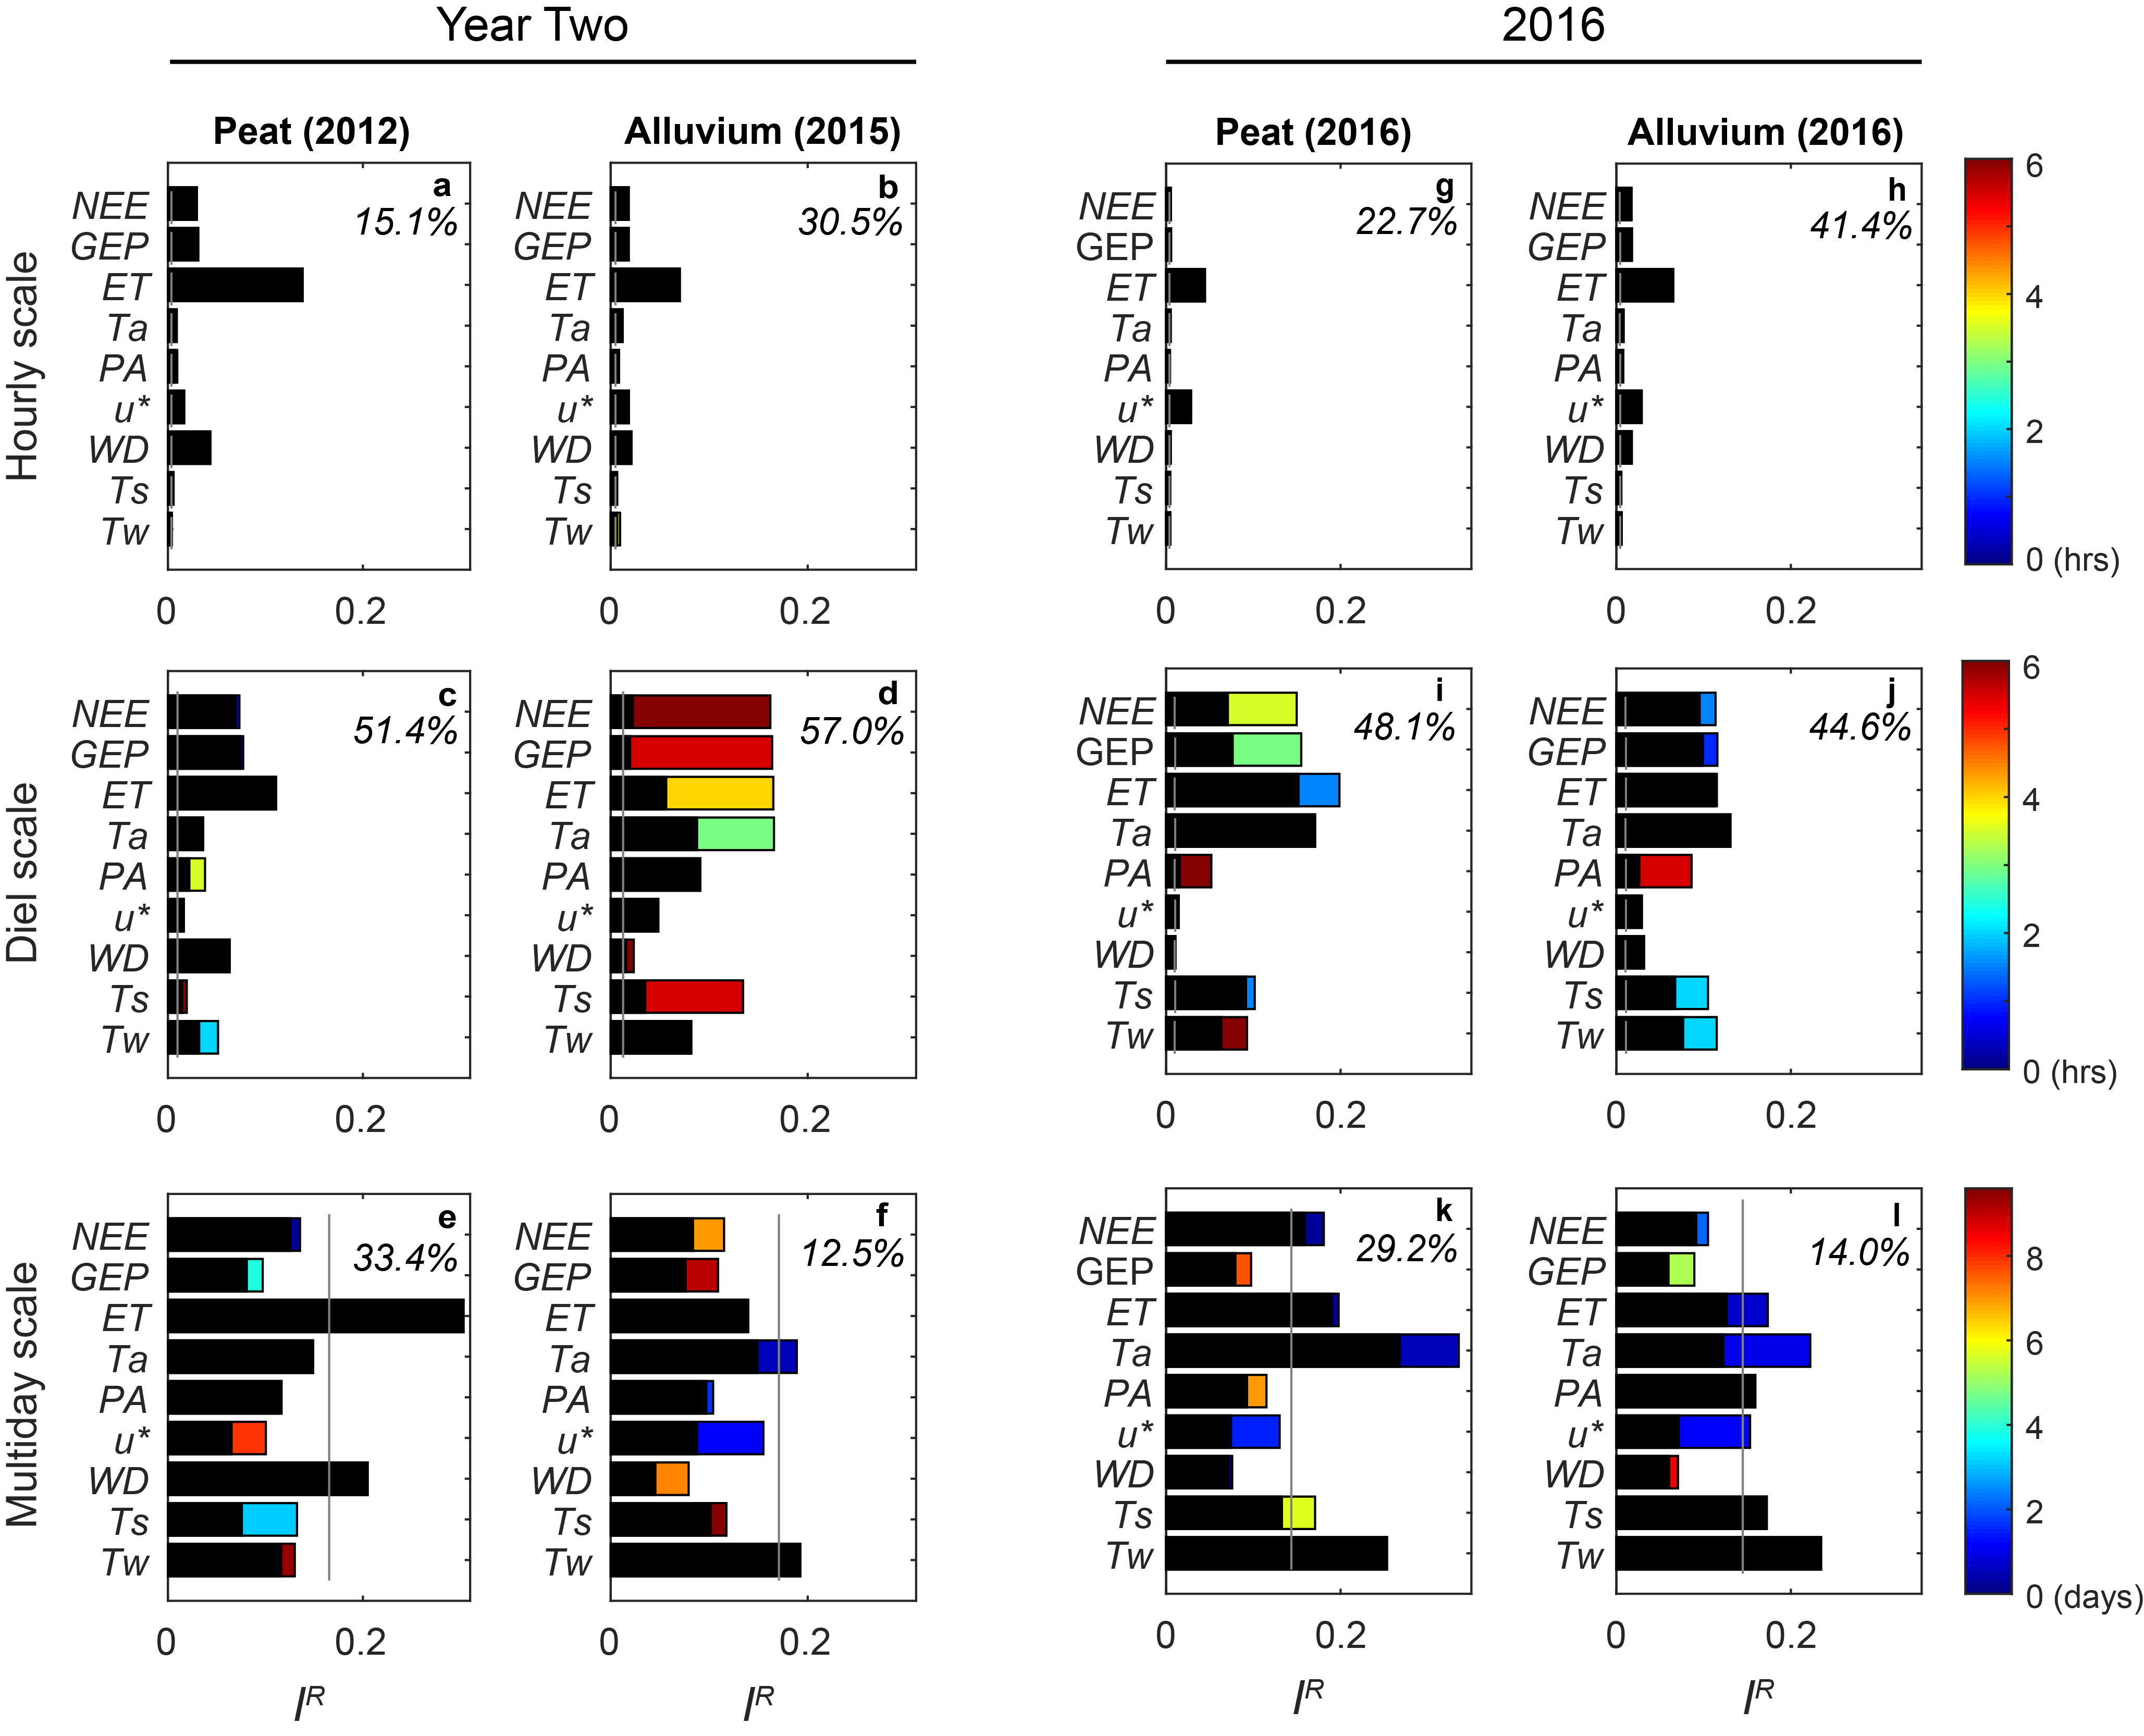
\includegraphics[keepaspectratio]{fig4.png}}
\caption{Mutual information (\emph{I\textsuperscript{R}}) shared between
methane flux (\emph{F\textsubscript{CH4}}) and biophysical variables at
multiple time scales for the peat and alluvium wetland (a-f) the second
year post-restoration (year two) when both wetlands were fully vegetated
and (g-l) during the 2016 growing season. Black bars indicate
\emph{I\textsuperscript{R}} at zero time lag, and colored extension
indicates maximum \emph{I\textsuperscript{R}} observed at the time lag
illustrated by the color scale. Vertical grey bars represent 95\%
confidence intervals generated from 1000 Monte Carlo random walks.
Italicized percentage inset on each panel indicates the percent of total
wavelet variance occurring at each time scale. Biophysical variables
include net ecosystem exchange (\emph{NEE}), gross ecosystem
photosynthesis (\emph{GEP}), evapotranspiration (\emph{ET}), air
temperature (\emph{T\textsubscript{a}}), air pressure (\emph{PA}),
friction velocity (\emph{u\(^\ast\)}), wind direction (\emph{WD}), soil
temperature (\emph{T\textsubscript{s}}), and water temperature
(\emph{T\textsubscript{w}}).}
\end{figure}

Alluvium wetland CH\textsubscript{4} flux patterns and interactions the
second year post-restoration (2015) were notably different from the peat
wetland. Alluvium wetland CH\textsubscript{4} fluxes were dominantly
coupled to physical processes at diel to multiday time scales, such as
temperature and atmospheric pressure (\emph{PA}) fluctuations (Fig.
4b,d,f), in contrast to the peat site where fluxes were primarily
coupled to plant processes (Fig. 4a,c,e). At the hourly scale,
CH\textsubscript{4} fluxes also shared most information with \emph{ET}
(Fig. 4b). At the diel scale, dominant interactions were observed with
\emph{PA} and water temperature (\emph{T\textsubscript{w}}) at no time
lag, and with \emph{T\textsubscript{a}} at a three hour lag (Fig. 4d).
Here, wetland maximum CH\textsubscript{4} fluxes were observed in the
late afternoon during atmospheric pressure lows (17:00 to 19:00 LT), and
this relationship displayed strong hysteresis (Fig. S2). This dominant
diel \emph{PA} interaction was not observed at the peat site (Fig. 4c).
Strong interactions were also observed between CH\textsubscript{4} flux
and \emph{GEP}/\emph{NEE}/\emph{ET}, but these interactions occurred at
a four to five hour time lag (Fig. 4d). These interactions can be
intuitively seen through the timing of fluxes, where peak \emph{NEE} and
\emph{ET} were observed mid-day, while peak CH\textsubscript{4} flux
occurred many hours later in the afternoon (Fig. S3). At the multiday
scale, alluvium CH\textsubscript{4} fluxes only shared significant
information with temperature variables (\emph{T\textsubscript{a}} and
\emph{T\textsubscript{w}}) (Fig. 4f). Hourly scale CH\textsubscript{4}
flux variability was more dominant at the alluvium wetland in year two,
as 57\% of total CH\textsubscript{4} flux signal variability occurred at
the diel scale, 30.5\% occurred at the hourly scale, and only 12.5\%
occurred at the multiday time scale (Fig. 4b,d,f).

By the 2016 growing season, CH\textsubscript{4} flux patterns and
interactions had converged across the peat and alluvium wetland sites.
Peak CH\textsubscript{4} fluxes were observed at roughly 15:00 LT at
both sites by 2016. This shift to an afternoon peak flux occurred in
2013 at the peat wetland, and patterns in flux timing were similar for
each year thereafter (Fig. S1). Both alluvium and peat sites were quite
different in terms of flux timing compared to the mature site, where
peak CH\textsubscript{4} flux occurred around noon most years (Fig. S1).

Scale-emergent controls of CH\textsubscript{4} flux were also very
similar between the alluvium and peat site during the 2016 growing
season (Fig. 4). For both sites, hourly CH\textsubscript{4} fluxes
exhibited dominant synchronous couplings to friction velocity
(\emph{u\(^\ast\)}) and \emph{ET} (Fig. 4g,h), and at the diel scale,
dominant interactions with CH\textsubscript{4} flux included
\emph{T\textsubscript{a}}, \emph{ET}, \emph{GEP}, and \emph{NEE} at both
wetlands (Fig. 4i,j). By 2016, dominant synchronous \emph{PA}
interactions observed at the alluvium site (Fig. 4d) were no longer
apparent, though \emph{PA} shared similar levels of information with
CH\textsubscript{4} flux at a 5-6 hour time lag (Fig. 4j). Multiday
scale interactions were also similar across sites, where significant
interactions with temperature variables (\emph{T\textsubscript{a}},
\emph{T\textsubscript{w}}, and \emph{T\textsubscript{s}}), as well as
\emph{ET}, were observed (Fig. 4k,l). There were some notable
differences between sites at the multiday scale, as CH\textsubscript{4}
flux also shared information with \emph{NEE} at the peat site (Fig. 4k),
and CH\textsubscript{4} flux shared information with \emph{PA} at the
alluvium site (Fig. 4l). At the peat wetland, most variability still
occurred at the diel scale (48.1\%), followed by the multiday (29.2\%)
and hourly (22.7\%) time scales (Fig. 4g,i,k). Most variability at the
alluvium wetland still occurred at the diel scale (44.6\%), followed
closely by the hourly scale (41.4\%), and much less variability occurred
at the multiday scale (14\%) (Fig. 4h,j,l).

\subsection{\texorpdfstring{What explains increasing alluvium
CH\textsubscript{4} fluxes with
time?}{What explains increasing alluvium CH4 fluxes with time?}}\label{what-explains-increasing-alluvium-ch4-fluxes-with-time}

To determine whether long-term increases in alluvium wetland
CH\textsubscript{4} emissions could be explained by common biophysical
drivers, we trained an empirical CH\textsubscript{4} flux model using
observations from a third independent, mature wetland site that was
restored in 1999 and is located \textasciitilde700m from the alluvium
wetland. The model predicted CH\textsubscript{4} fluxes based on nine
common biophysical drivers identified here and in Sturtevant \emph{et
al.} (\citeproc{ref-sturtevant_identifying_2016}{2016}), including
\emph{PAR}, \emph{T\textsubscript{a}}, \emph{PA}, \emph{u\(^\ast\)},
\emph{GEP}, \emph{ER}, a greenness index (\emph{GCC}), and vapor
pressure deficit. We fit a GAM using penalized regression splines to
capture non-linear relationships, and the model was fit to four years of
daily flux data from the mature wetland (\emph{n} = 1464), where
ten-fold cross-validation was used to tune the model for best fit (final
model - no feature selection; \emph{r\textsuperscript{2}} = 0.77).

The trained GAM performed relatively well against observed peat wetland
CH\textsubscript{4} fluxes (\emph{r\textsuperscript{2}} = 0.6). Within
each year (2012 - 2017), residual CH\textsubscript{4} fluxes were
distributed around zero and skewed slightly negative, indicating some
overestimation in predicted fluxes. The model residual interquartile
range (IQR) always overlapped with zero, except for 2017 when multiple
disturbance events reduced CO2 and CH4 fluxes from the peat wetland
(Fig. 5).

The GAM performance against the alluvium wetland was notably worse
(\emph{r\textsuperscript{2}} = 0.34) and was highly variable across
years (Fig. 5). Observed alluvium CH\textsubscript{4} fluxes were
substantially lower than model predictions the second year following
restoration (2015), as indicated by negative residuals when the IQR did
not cross zero (Fig. 5). This strong negative skew reduced in subsequent
years, and by 2017 there was no observed bias in model
CH\textsubscript{4} residuals (Fig. 5). The GAM predicted 72.59\% of
observed variance in 2017, indicating more accurate CH\textsubscript{4}
flux predictions as the alluvium wetland developed.

Model over-prediction in early years at the alluvium wetland suggests
that other factors, not measured directly by the eddy covariance tower,
could have inhibited initial CH\textsubscript{4} emissions. Though our
soil data was collected during a single sampling in 2017, we can
substitute depth for time to track changes in soil properties over this
time period. If we assume the parent horizon is indicative of soils at
the time of restoration and the accreted horizon is indicative of the
current state of wetland soils, we observe a significant increase in
soil pH (Fig. 2d) and a shift towards more Fe in its reduced form
(Fe\textsuperscript{2+}) as alluvium wetland soils developed (Fig. 2b).

\begin{figure}
\centering
\pandocbounded{\includegraphics[keepaspectratio]{manuscript_files/figure-latex/fig5-1.pdf}}
\caption{Residual CH\textsubscript{4} flux (\emph{F\textsubscript{CH4}};
mg C m\textsuperscript{-2} d\textsuperscript{-1}) for both recently
restored wetlands using an empirical model trained on
CH\textsubscript{4} fluxes from a mature, stable state wetland site
restored in 1999. A generalized additive model was trained on four years
of daily CH\textsubscript{4} fluxes using nine common biophysical
drivers (see Results for details) and ten-fold cross validation. First
year fluxes were omitted from residual analysis because the model was
trained on a fully vegetated, mature wetland.}
\end{figure}

\subsection{Implications for restored wetland GHG
emissions}\label{implications-for-restored-wetland-ghg-emissions}

Methane emissions from the alluvium wetland increased steadily with
time. This stands in contrast to the trend of reducing
CH\textsubscript{4} emissions in recent years at the other wetlands,
where annual CH\textsubscript{4} budgets from the peat and mature
wetland covaried and were not statistically different from one another
from 2014 to 2017 (Fig. 6a). By 2017, annual CH\textsubscript{4} fluxes
from the alluvium wetland exceeded emissions from the peat and mature
wetlands, though were significantly lower than emissions from the other
sites in the previous two years (2015 and 2016) (Fig. 6a). In 2015,
alluvium CH\textsubscript{4} budgets were 48-50\% the magnitude of the
other sites, and in 2016 the alluvium CH\textsubscript{4} budget was
75-78\% of the other sites (Fig. 6a). Reduced CH\textsubscript{4}
budgets in 2015 and 2016 initially corresponded to neutral GHG emissions
from the alluvium wetland (Fig. 6b); however, by 2017 the alluvium GHG
budget was positive and trended larger than the other sites (Fig. 6b).
Conversely, the peat and mature wetlands were both GHG sources from 2014
to 2016, and GHG neutral in 2017 (Fig. 6b). Soil iron content
(extractable and poorly crystalline Fe) was similar across parent
horizons of peat and mature wetlands (Tukey's HSD, \emph{P}
\textgreater{} 0.5) (Fig. S5), though soil C concentrations were
significantly higher at the mature wetland compared to the peat and
alluvium sites (Tukey's HSD, \emph{P} \textless{} 0.01) (Fig. S5). These
wetlands experienced similar climatic and hydrologic conditions over
this time period (Fig. S3).

\begin{figure}
\centering
\pandocbounded{\includegraphics[keepaspectratio]{manuscript_files/figure-latex/fig6-1.pdf}}
\caption{Annual CH\textsubscript{4} flux (\emph{F\textsubscript{CH4}})
and greenhouse gas budget (GHG) across the two recently restored peat
and alluvium wetlands, as well as the mature wetland restored on peat
soils. Annual GHG balance is computed from annual
\emph{F\textsubscript{CH4}} and \emph{NEE} budgets using the sustained
global warming potential for CH\textsubscript{4}
(\citeproc{ref-neubauer_moving_2015}{Neubauer \& Megonigal, 2015}).}
\end{figure}

\section{Discussion}\label{discussion}

Our results suggest that soil type, a legacy of the pre-drainage
landscape, influences ecosystem-scale CH\textsubscript{4} emissions from
restored wetlands. We observed substantially lower CH\textsubscript{4}
emissions for multiple years following restoration from a wetland
restored on alluvium compared to peat soils; however,
CH\textsubscript{4} flux magnitudes converged across the wetlands three
years post-restoration (Fig. 3a). Initial CH\textsubscript{4} flux
differences were not driven by variable climate or hydrologic forcing,
as these wetlands experienced similar meteorologic conditions and both
remained inundated year-round (Fig. 3). Additionally, alluvium
\emph{NEE} was often similar to, or larger than, \emph{NEE} from the
peat site (Fig. 3b), demonstrating that differences in
CH\textsubscript{4} flux were not due to covariation with other factors
broadly affecting wetland GHG exchange. Soil Fe, C content, and pH are
edaphic factors known to influence CH\textsubscript{4} production rates
in soil (\citeproc{ref-teh_suppression_2008}{Teh \emph{et al.}, 2008};
\citeproc{ref-ye_ph_2012}{Ye \emph{et al.}, 2012};
\citeproc{ref-bridgham_methane_2013}{Bridgham \emph{et al.}, 2013}).
Soil C has been shown to be a strong proxy for CH\textsubscript{4}
emissions from rewetted peatlands on these islands
(\citeproc{ref-ye_soil_2016}{Ye \emph{et al.}, 2016}); however, soil C
did not vary between wetlands at the time of restoration, as we observed
similar C concentrations in parent horizons across both sites (Fig. 2).
Additionally, soil C does not appear to drive CH\textsubscript{4}
emissions more broadly across the wetland network, as annual
CH\textsubscript{4} fluxes did not vary across peat and mature wetlands
(Fig. 6), though their soil C concentrations varied substantially (Fig.
S5). These observations suggest that reduced CH\textsubscript{4}
emissions may instead be related to the acidic conditions and high Fe
content in alluvium soils (Fig. 2).

Alluvium soil Fe concentrations were comparable to tropical forest soils
where microbial Fe reduction is known to inhibit CH\textsubscript{4}
production. Yang \& Liptzin (\citeproc{ref-yang_high_2015}{2015})
observed mean Fe concentrations of 23.6 mg Fe g\textsuperscript{-1} soil
in forest soils where Teh \emph{et al.}
(\citeproc{ref-teh_suppression_2008}{2008}) had previously documented
suppression of methanogenesis by microbial Fe reduction. Alluvium
wetland Fe concentrations were similar (21.76 \(\pm\) 5.88 mg Fe
g\textsuperscript{-1} soil; \emph{n} = 30), demonstrating that Fe
concentrations were within the range where microbial Fe reduction
inhibits methanogenesis. In contrast to upland humid tropical forests
where most Fe is found in poorly crystalline form
(\citeproc{ref-dubinsky_tropical_2010}{Dubinsky \emph{et al.}, 2010};
\citeproc{ref-hall_reducing_2015}{Hall \& Silver, 2015};
\citeproc{ref-yang_high_2015}{Yang \& Liptzin, 2015}), poorly
crystalline Fe concentrations were roughly two orders of magnitude lower
than the HCl-extractable Fe pool across the wetland sites. Poorly
crystalline Fe pools are readily reducible by soil microbes
(\citeproc{ref-hyacinthe_reactive_2006}{Hyacinthe \emph{et al.}, 2006};
\citeproc{ref-hall_reducing_2015}{Hall \& Silver, 2015}), and depletion
of these pools suggests high activity by microbial Fe reducers in
wetland soils (\citeproc{ref-weiss_geochemical_2004}{Weiss \emph{et
al.}, 2004}). Depleted reducible Fe pools in wetlands relative to upland
systems is expected, as stable anoxic wetland conditions promotes
extended Fe reducer activity and utilization of poorly crystalline Fe
pools (\citeproc{ref-teh_suppression_2008}{Teh \emph{et al.}, 2008};
\citeproc{ref-dubinsky_tropical_2010}{Dubinsky \emph{et al.}, 2010}).
Our observations of high Fe concentrations, low poorly crystalline Fe
pools, and low CH\textsubscript{4} fluxes at the alluvium wetland all
suggest that Fe reduction is a dominant form of anaerobic respiration
capable of inhibiting CH\textsubscript{4} flux at this site. Differences
in soil pH may also contribute to observed flux differences; however,
strong inhibition of methanogenesis tends to occur at pH values below 5
(\citeproc{ref-dunfield_methane_1993}{Dunfield \emph{et al.}, 1993};
\citeproc{ref-kotsyurbenko_shift_2007}{Kotsyurbenko \emph{et al.},
2007}; \citeproc{ref-ye_ph_2012}{Ye \emph{et al.}, 2012}), while we
observed mean pH values of 5.27 in the alluvium parent soils. Further
incubation experiments are warranted to disentangle the direct mechanism
reducing CH\textsubscript{4} fluxes, as pH, Fe cycling, and redox state
co-vary in inundated soils
(\citeproc{ref-gotoh_transformation_1974}{Gotoh \& Patrick, 1974}).

The question remains: Why did CH\textsubscript{4} flux differences
between the peat and alluvium wetlands disappear with time? Our
empirical model based on dominant biophysical drivers of mature wetland
CH\textsubscript{4} flux, including \emph{NEE}, \emph{GEP}, and
\emph{ER}, could not explain why alluvium CH\textsubscript{4} fluxes
were initially low relative to the other sites (Fig. 6), suggesting that
other factors might be responsible for reduced fluxes in early
succession. We suspect this is related to soil development over time, as
we observed increases in reduced ferrous iron (Fe\textsuperscript{2+})
and a shift toward less acidic conditions in alluvium accreted soil
compared to the underlying parent soil (Fig. 2). Increases in
Fe\textsuperscript{2+} and pH suggest more reduced conditions favorable
to methanogenesis in the accreted soils where poorly crystalline Fe
pools are depleted faster than they are replenished. Acidic soils are
also known to directly inhibit methanogenesis
(\citeproc{ref-dunfield_methane_1993}{Dunfield \emph{et al.}, 1993};
\citeproc{ref-ye_ph_2012}{Ye \emph{et al.}, 2012}) and alter methanogen
community structure (\citeproc{ref-kotsyurbenko_shift_2007}{Kotsyurbenko
\emph{et al.}, 2007}), though often in more acidic conditions as
described above. This interaction between less acidic and more reduced
conditions could enhance CH\textsubscript{4} production rates in the
newly accreted soils as alluvium wetlands develop.

Initial differences in wetland biophysical CH\textsubscript{4} drivers
the second year following restoration provides a further line of
evidence that alluvium CH\textsubscript{4} fluxes were inhibited by Fe
reduction. Alluvium CH\textsubscript{4} fluxes were decoupled from plant
processes across multiple scales compared to the peat site. Peat
CH\textsubscript{4} fluxes were more dominantly coupled to plant
processes, such as \emph{GEP} and \emph{ET} (Fig. 4), while alluvium
CH\textsubscript{4} fluxes were more dominantly coupled to physical
transport (pressure pumping; Fig. S2) and temperature, which dictates
CH\textsubscript{4} production rates in bulk soil
(\citeproc{ref-yvon-durocher_methane_2014}{Yvon-Durocher \emph{et al.},
2014}). This decoupling from plant-derived substrates (\emph{GEP}) and
transport pathways (\emph{ET}) suggests that less CH\textsubscript{4}
was derived from plant exudates in the rhizosphere. Oxygen is released
into wetland soils through plant roots, and the rhizosphere is typically
an area of high CH\textsubscript{4} oxidation
(\citeproc{ref-van_der_nat_seasonal_1998}{Nat \& Middelburg, 1998};
\citeproc{ref-laanbroek_methane_2010}{Laanbroek, 2010}). The wetland
rhizosphere is also a hotspot of microbial Fe oxidation and reduction
given the co-occurrence of oxic-anoxic conditions
(\citeproc{ref-weiss_enumeration_2003}{Weiss \emph{et al.}, 2003}). For
sites with higher Fe, such as the alluvium wetland, CH\textsubscript{4}
fluxes might be more decoupled from plant substrates (\emph{GEP}) and
transport pathways (\emph{ET}) where rhizosphere methanogenesis is
further inhibited by active Fe redox cycling
(\citeproc{ref-laanbroek_methane_2010}{Laanbroek, 2010}). Such
inhibition of methanogenesis has been observed in microcosm and
incubation studies, where oxygen input via plant roots re-oxidizes
ferrous Fe and further suppresses CH\textsubscript{4} production in the
root zone (\citeproc{ref-roden_organic_1996}{Roden \& Wetzel, 1996};
\citeproc{ref-frenzel_rice_1999}{Frenzel \emph{et al.}, 1999};
\citeproc{ref-sutton-grier_plant_2011}{Sutton-Grier \& Megonigal,
2011}). Anaerobic microbial re-oxidation of Fe coupled to
NO\textsubscript{3}\textsuperscript{-} reduction is also known to occur
in wetland sediments (\citeproc{ref-weber_anaerobic_2006}{Weber \emph{et
al.}, 2006}) and may be relevant to Fe cycling in these wetlands if
significant NO\textsubscript{3}\textsuperscript{-} enters the system
from upslope agriculture.

Conversely, we might expect to see stronger couplings to plant processes
for sites with lower soil Fe concentrations, as we observe for the peat
wetland (Fig. 4). Sturtevant \emph{et al.}
(\citeproc{ref-sturtevant_identifying_2016}{2016}) also demonstrated
strong diel CH\textsubscript{4} couplings to \emph{ET} and \emph{GEP} at
the mature wetland where soil Fe concentrations are low relative to the
alluvium site (Fig. S5). Hatala \emph{et al.}
(\citeproc{ref-hatala_gross_2012}{2012a}) and Knox \emph{et al.}
(\citeproc{ref-knox_biophysical_2016}{2016}) found that diel patterns in
CH\textsubscript{4} fluxes from Delta rice were driven by \emph{GEP},
rather than temperature, because peak CH\textsubscript{4} flux lagged
\emph{GEP} by \textasciitilde1-2 hrs and led maximum soil temperature.
We saw a very different dynamic at the alluvium wetland where peak
CH\textsubscript{4} flux occurred late in the afternoon, many hours
after peak \emph{GEP}, \emph{ET}, and \emph{T\textsubscript{a}}, and was
instead synchronously coupled to \emph{PA} and \emph{T\textsubscript{w}}
fluctuations (Fig. 4). These dynamics further suggest decoupling from
recent plant-derived C substrates and transport pathways at the alluvium
wetland, with more dominant couplings to physical transport and drivers
of bulk soil methanogenesis, as expected if rhizosphere
CH\textsubscript{4} production was inhibited by active Fe redox.

Convergence of CH\textsubscript{4} flux biophysical drivers with time
further suggests that as soils develop CH\textsubscript{4} fluxes and
controls become more similar across wetland types. The hierarchy of
dominant biophysical drivers and lagged effects were quite similar
across the peat and alluvium wetlands in 2016 (Fig. 4g-l) compared to
the second year when flux-driver relationships were very different
across the two systems (Fig. 4a-f). Here, the most notable shift
occurred at the alluvium wetland, where CH\textsubscript{4} fluxes were
strongly coupled to physical processes in the second year (Fig. 4b,d,f)
and by 2016 fluxes were also coupled to plant processes across multiple
scales, such as \emph{NEE}, \emph{GEP}, and \emph{ET} (Fig. 4h,j,l). The
mature wetland GAM was also better able to predict alluvium wetland
CH\textsubscript{4} fluxes as this shift occurred (Fig. 5), further
suggesting stronger couplings to plant processes as the alluvium wetland
and its soils developed.

Differences in controls across scale are discussed in more detail in
Sturtevant \emph{et al.}
(\citeproc{ref-sturtevant_identifying_2016}{2016}), but we find
short-term (hourly) variability in CH\textsubscript{4} flux is
influenced by transport mechanisms (\emph{ET} and \emph{u\(^\ast\)}),
diel variation is more dictated by plant processes and temperature
(\emph{NEE}, \emph{GEP}, \emph{ET}, and \emph{T\textsubscript{a}}),
while weekly to monthly variation is driven by temperature oscillations.
Surprisingly, much more flux variability occurred at the multiday scale
for the peat wetland than the alluvium wetland, and this pattern was
consistent over time (Fig. 4). While the driver of this inter-site
variation is not clear, it demonstrates that eddy covariance is
particularly well-suited to ecosystem CH\textsubscript{4} flux
measurements. Non-automated chamber measurement campaigns could easily
under-sample important modes of CH\textsubscript{4} flux variation,
particularly if dominant modes of variation change across wetlands
distributed over small spatial scales.

Overall, our findings demonstrate that soil type impacts ecosystem-scale
CH\textsubscript{4} emissions and GHG budgets from restored wetlands on
annual time scales. We found that differences in CH\textsubscript{4}
flux between alluvium and peat wetlands were pronounced for the first
few years following restoration, causing significant reductions in net
GHG emissions from the wetland restored on alluvium soils (Fig. 6).
Initial differences were most likely due to high Fe content within
alluvium soils, as Fe concentrations were in the range where inhibition
of methanogenesis is known to occur
(\citeproc{ref-teh_suppression_2008}{Teh \emph{et al.}, 2008}), and soil
C, another common driver of CH\textsubscript{4} emissions
(\citeproc{ref-ye_soil_2016}{Ye \emph{et al.}, 2016}), did not vary
across sites at the initial point of restoration. However, reduced
CH\textsubscript{4} emissions and GHG budgets faded with time, likely
due to the development of more reduced, less acidic conditions favorable
to CH\textsubscript{4} production within accreted alluvium sediments.
Wetland restoration projects have a lifetime of multiple decades (over
20 years for the mature wetland), so these transient reductions in
CH\textsubscript{4} flux are likely of low importance from a policy or
management perspective because any GHG benefit of restoring wetlands on
alluvium soil are lost within a few years of restoration. This work
illustrates a transient influence of soil properties on long-term
wetland GHG emissions, which improves our understanding of site
selection consequences to GHG emissions from restored wetlands.

\section{Acknowledgements}\label{acknowledgements}

This research was supported in part by the U.S. Department of Energy's
Office of Science and its funding of Ameriflux core sites (Ameriflux
contract 7079856), and the California Division of Fish and Wildlife,
through a contract of the California Department of Water Resources
(Award 4600011240). We thank three anonymous reviewers for their
constructive feedback on drafts of this manuscript.

\section*{References}\label{references}
\addcontentsline{toc}{section}{References}

\phantomsection\label{refs}
\begin{CSLReferences}{1}{0}
\bibitem[\citeproctext]{ref-ali_silicate_2009}
Ali MA, Lee CH, Lee YB, Kim PJ (2009)
\href{https://doi.org/10.1016/j.agee.2009.02.014}{Silicate fertilization
in no-tillage rice farming for mitigation of methane emission and
increasing rice productivity}. \emph{Agriculture, Ecosystems \&
Environment}, \textbf{132}, 16--22.

\bibitem[\citeproctext]{ref-angle_methanogenesis_2017}
Angle JC, Morin TH, Solden LM et al. (2017)
\href{https://doi.org/10.1038/s41467-017-01753-4}{Methanogenesis in
oxygenated soils is a substantial fraction of wetland methane
emissions}. \emph{Nature Communications}, \textbf{8}, 1567.

\bibitem[\citeproctext]{ref-atwater1980tidal}
Atwater BF, Belknap DF (1980) Tidal-wetland deposits of the
{Sacramento-San Joaquin Delta, California}. In: \emph{Quaternary
depositional environments of the pacific coast: Pacific coast
paleogeography symposium 4.} (eds Field ME, Bouma AH, Coburn IP, Douglas
RG, C IJ), pp. 89--103. The Pacific Section of the Society of Economic
Paleontologists; Mineralogists, Los Angeles, California.

\bibitem[\citeproctext]{ref-atwater1979history}
Atwater BF, Conrad S, Dowden JN, Hedel CW, MacDonald RL, Savage W (1979)
History, landforms, and vegetation of the estuary's tidal marshes. In:
\emph{{San Francisco Bay}: The urbanized estuary: Investigations into
the natural history of {San Francisco Bay and Delta} with reference to
the influence of man.} (ed Conomos TJ), pp. 347--386. AAAS Pacific
Division, San Francisco, California.

\bibitem[\citeproctext]{ref-gridExtra}
Auguie B (2016)
\emph{\emph{\href{https://CRAN.R-project.org/package=gridExtra}{gridExtra:
Miscellaneous functions for "grid" graphics}}}.

\bibitem[\citeproctext]{ref-baldocchi_does_2015}
Baldocchi D, Sturtevant C, Fluxnet Contributors (2015)
\href{https://doi.org/10.1016/j.agrformet.2015.03.010}{Does day and
night sampling reduce spurious correlation between canopy photosynthesis
and ecosystem respiration?} \emph{Agricultural and Forest Meteorology},
\textbf{207}, 117--126.

\bibitem[\citeproctext]{ref-bridgham_methane_2013}
Bridgham SD, Cadillo-Quiroz H, Keller JK, Zhuang Q (2013)
\href{https://doi.org/10.1111/gcb.12131}{Methane emissions from
wetlands: Biogeochemical, microbial, and modeling perspectives from
local to global scales}. \emph{Global Change Biology}, \textbf{19},
1325--1346.

\bibitem[\citeproctext]{ref-brown_evidence_2014}
Brown MG, Humphreys ER, Moore TR, Roulet NT, Lafleur PM (2014)
\href{https://doi.org/10.1002/2013JG002576}{Evidence for a nonmonotonic
relationship between ecosystem-scale peatland methane emissions and
water table depth}. \emph{Journal of Geophysical Research:
Biogeosciences}, \textbf{119}, 2013JG002576.

\bibitem[\citeproctext]{ref-bubier_ecological_1994}
Bubier JL, Moore TR (1994)
\href{https://doi.org/10.1016/0169-5347(94)90309-3}{An ecological
perspective on methane emissions from northern wetlands}. \emph{Trends
in Ecology \& Evolution}, \textbf{9}, 460--464.

\bibitem[\citeproctext]{ref-chamberlain_underlying_2015}
Chamberlain SD, Boughton EH, Sparks JP (2015)
\href{https://doi.org/10.1007/s10021-015-9873-x}{Underlying ecosystem
emissions exceed cattle-emitted methane from subtropical lowland
pastures}. \emph{Ecosystems}, \textbf{18}, 933--945.

\bibitem[\citeproctext]{ref-chamberlain_influence_2016}
Chamberlain SD, Gomez-Casanovas N, Walter MT et al. (2016)
\href{https://doi.org/10.1002/2015JG003283}{Influence of transient
flooding on methane fluxes from subtropical pastures}. \emph{Journal of
Geophysical Research: Biogeosciences}, \textbf{121}, 2015JG003283.

\bibitem[\citeproctext]{ref-chamberlain_evaluation_2017}
Chamberlain SD, Verfaillie J, Eichelmann E, Hemes KS, Baldocchi DD
(2017b) \href{https://doi.org/10.1007/s10546-017-0275-9}{Evaluation of
density corrections to methane fluxes measured by open-path eddy
covariance over contrasting landscapes}. \emph{Boundary-Layer
Meteorology}, \textbf{165}, 197--210.

\bibitem[\citeproctext]{ref-chamberlain_impact_2017}
Chamberlain SD, Groffman PM, Boughton EH, Gomez-Casanovas N, DeLucia EH,
Bernacchi CJ, Sparks JP (2017a)
\href{https://doi.org/10.1002/eap.1514}{The impact of water management
practices on subtropical pasture methane emissions and ecosystem service
payments}. \emph{Ecological Applications}, \textbf{27}, 1199--1209.

\bibitem[\citeproctext]{ref-chu_net_2014}
Chu H, Chen J, Gottgens JF, Ouyang Z, John R, Czajkowski K, Becker R
(2014) \href{https://doi.org/10.1002/2013JG002520}{Net ecosystem methane
and carbon dioxide exchanges in a lake erie coastal marsh and a nearby
cropland}. \emph{Journal of Geophysical Research: Biogeosciences},
\textbf{119}, 2013JG002520.

\bibitem[\citeproctext]{ref-conrad_global_2009}
Conrad R (2009)
\href{https://doi.org/10.1111/j.1758-2229.2009.00038.x}{The global
methane cycle: Recent advances in understanding the microbial processes
involved}. \emph{Environmental Microbiology Reports}, \textbf{1},
285--292.

\bibitem[\citeproctext]{ref-conservation_international_blue}
Conservation International (2017) The {Blue} {Carbon} {Initiative}.

\bibitem[\citeproctext]{ref-detto_soil_2006}
Detto M, Montaldo N, Albertson JD, Mancini M, Katul G (2006)
\href{https://doi.org/10.1029/2005WR004693}{Soil moisture and vegetation
controls on evapotranspiration in a heterogeneous mediterranean
ecosystem on sardinia, italy}. \emph{Water Resources Research},
\textbf{42}, W08419.

\bibitem[\citeproctext]{ref-deverel_historic_2010}
Deverel SJ, Leighton DA (2010)
\href{http://escholarship.org/uc/item/7xd4x0xw}{Historic, recent, and
future subsidence, {Sacramento-San Joaquin Delta, California, USA}}.
\emph{San Francisco Estuary and Watershed Science}, \textbf{8}, 1--23.

\bibitem[\citeproctext]{ref-drexler_peat_2011}
Drexler JZ (2011) \href{https://doi.org/10.1007/s12237-011-9393-7}{Peat
formation processes through the millennia in tidal marshes of the
sacramento--san joaquin delta, california, {USA}}. \emph{Estuaries and
Coasts}, \textbf{34}, 900.

\bibitem[\citeproctext]{ref-drexler_peat_2009}
Drexler JZ, Fontaine CS de, Brown TA (2009)
\href{https://doi.org/10.1007/s12237-009-9202-8}{Peat accretion
histories during the past 6,000 years in marshes of the sacramento--san
joaquin delta, {CA}, {USA}}. \emph{Estuaries and Coasts}, \textbf{32},
871--892.

\bibitem[\citeproctext]{ref-dubinsky_tropical_2010}
Dubinsky EA, Silver WL, Firestone MK (2010)
\href{https://doi.org/10.1890/09-1365.1}{Tropical forest soil microbial
communities couple iron and carbon biogeochemistry}. \emph{Ecology},
\textbf{91}, 2604--2612.

\bibitem[\citeproctext]{ref-dunfield_methane_1993}
Dunfield P, knowles R, Dumont R, Moore TR (1993)
\href{https://doi.org/10.1016/0038-0717(93)90130-4}{Methane production
and consumption in temperate and subarctic peat soils: Response to
temperature and {pH}}. \emph{Soil Biology and Biochemistry},
\textbf{25}, 321--326.

\bibitem[\citeproctext]{ref-forbrich_cross-evaluation_2011}
Forbrich I, Kutzbach L, Wille C, Becker T, Wu J, Wilmking M (2011)
\href{https://doi.org/10.1016/j.agrformet.2011.02.006}{Cross-evaluation
of measurements of peatland methane emissions on microform and ecosystem
scales using high-resolution landcover classification and source weight
modelling}. \emph{Agricultural and Forest Meteorology}, \textbf{151},
864--874.

\bibitem[\citeproctext]{ref-frenzel_rice_1999}
Frenzel P, Bosse U, Janssen PH (1999)
\href{https://doi.org/10.1016/S0038-0717(98)00144-8}{Rice roots and
methanogenesis in a paddy soil: Ferric iron as an alternative electron
acceptor in the rooted soil}. \emph{Soil Biology and Biochemistry},
\textbf{31}, 421--430.

\bibitem[\citeproctext]{ref-goodrich_overriding_2015}
Goodrich JP, Campbell DI, Roulet NT, Clearwater MJ, Schipper LA (2015)
\href{https://doi.org/10.1002/2014JG002844}{Overriding control of
methane flux temporal variability by water table dynamics in a southern
hemisphere, raised bog}. \emph{Journal of Geophysical Research:
Biogeosciences}, \textbf{120}, 2014JG002844.

\bibitem[\citeproctext]{ref-gotoh_transformation_1974}
Gotoh S, Patrick WH (1974)
\href{https://doi.org/10.2136/sssaj1974.03615995003800010024x}{Transformation
of iron in a waterlogged soil as influenced by redox potential and {pH}
1}. \emph{Soil Science Society of America Journal}, \textbf{38}, 66--71.

\bibitem[\citeproctext]{ref-graham_soil_2010}
Graham RC, O'Geen AT (2010)
\href{https://doi.org/10.1016/j.geoderma.2009.05.018}{Soil mineralogy
trends in california landscapes}. \emph{Geoderma}, \textbf{154},
418--437.

\bibitem[\citeproctext]{ref-lubridate}
Grolemund G, Wickham H (2011)
\href{http://www.jstatsoft.org/v40/i03/}{Dates and times made easy with
{lubridate}}. \emph{Journal of Statistical Software}, \textbf{40},
1--25.

\bibitem[\citeproctext]{ref-hall_iron_2013}
Hall SJ, Silver WL (2013) \href{https://doi.org/10.1111/gcb.12229}{Iron
oxidation stimulates organic matter decomposition in humid tropical
forest soils}. \emph{Global Change Biology}, \textbf{19}, 2804--2813.

\bibitem[\citeproctext]{ref-hall_reducing_2015}
Hall SJ, Silver WL (2015)
\href{https://doi.org/10.1007/s10533-015-0120-5}{Reducing conditions,
reactive metals, and their interactions can explain spatial patterns of
surface soil carbon in a humid tropical forest}. \emph{Biogeochemistry},
\textbf{125}, 149--165.

\bibitem[\citeproctext]{ref-hansson_conflicting_2005}
Hansson L-A, Brönmark C, Anders Nilsson P, Åbjörnsson K (2005)
\href{https://doi.org/10.1111/j.1365-2427.2005.01352.x}{Conflicting
demands on wetland ecosystem services: Nutrient retention, biodiversity
or both?} \emph{Freshwater Biology}, \textbf{50}, 705--714.

\bibitem[\citeproctext]{ref-hatala_greenhouse_2012}
Hatala JA, Detto M, Sonnentag O, Deverel SJ, Verfaillie J, Baldocchi DD
(2012b) \href{https://doi.org/10.1016/j.agee.2012.01.009}{Greenhouse gas
({CO}\(_2\), {CH}\(_4\), {H\(_2\)O}) fluxes from drained and flooded
agricultural peatlands in the {Sacramento-San Joaquin Delta}}.
\emph{Agriculture, Ecosystems \& Environment}, \textbf{150}, 1--18.

\bibitem[\citeproctext]{ref-hatala_gross_2012}
Hatala JA, Detto M, Baldocchi DD (2012a)
\href{https://doi.org/10.1029/2012GL051303}{Gross ecosystem
photosynthesis causes a diurnal pattern in methane emission from rice}.
\emph{Geophysical Research Letters}, \textbf{39}, L06409.

\bibitem[\citeproctext]{ref-hendriks_full_2007}
Hendriks DMD, Huissteden J van, Dolman AJ, Molen MK van der (2007)
\href{https://doi.org/10.5194/bg-4-411-2007}{The full greenhouse gas
balance of an abandoned peat meadow}. \emph{Biogeosciences}, \textbf{4},
411--424.

\bibitem[\citeproctext]{ref-hendriks_multi-technique_2010}
Hendriks DMD, Huissteden J van, Dolman AJ (2010)
\href{https://doi.org/10.1016/j.agrformet.2009.06.017}{Multi-technique
assessment of spatial and temporal variability of methane fluxes in a
peat meadow}. \emph{Agricultural and Forest Meteorology}, \textbf{150},
757--774.

\bibitem[\citeproctext]{ref-holm_ecosystem_2016}
Holm GO, Perez BC, McWhorter DE, Krauss KW, Johnson DJ, Raynie RC,
Killebrew CJ (2016)
\href{https://doi.org/10.1007/s13157-016-0746-7}{Ecosystem level methane
fluxes from tidal freshwater and brackish marshes of the mississippi
river delta: Implications for coastal wetland carbon projects}.
\emph{Wetlands}, \textbf{36}, 401--413.

\bibitem[\citeproctext]{ref-hsieh_approximate_2000}
Hsieh C-I, Katul G, Chi T (2000)
\href{https://doi.org/10.1016/S0309-1708(99)00042-1}{An approximate
analytical model for footprint estimation of scalar fluxes in thermally
stratified atmospheric flows}. \emph{Advances in Water Resources},
\textbf{23}, 765--772.

\bibitem[\citeproctext]{ref-hyacinthe_reactive_2006}
Hyacinthe C, Bonneville S, Van Cappellen P (2006)
\href{https://doi.org/10.1016/j.gca.2006.05.018}{Reactive iron({III}) in
sediments: Chemical versus microbial extractions}. \emph{Geochimica et
Cosmochimica Acta}, \textbf{70}, 4166--4180.

\bibitem[\citeproctext]{ref-jackel_suppression_2000}
Jäckel U, Schnell S (2000)
\href{https://doi.org/10.1016/S0038-0717(00)00094-8}{Suppression of
methane emission from rice paddies by ferric iron fertilization}.
\emph{Soil Biology and Biochemistry}, \textbf{32}, 1811--1814.

\bibitem[\citeproctext]{ref-caret}
Jed Wing MKuhnC from, Weston S, Williams A et al. (2017)
\emph{\emph{\href{https://CRAN.R-project.org/package=caret}{Caret:
Classification and regression training}}}.

\bibitem[\citeproctext]{ref-ggpubr}
Kassambara A (2017)
\emph{\emph{\href{https://CRAN.R-project.org/package=ggpubr}{Ggpubr:
'ggplot2' based publication ready plots}}}.

\bibitem[\citeproctext]{ref-kirschke_three_2013}
Kirschke S, Bousquet P, Ciais P et al. (2013)
\href{https://doi.org/10.1038/ngeo1955}{Three decades of global methane
sources and sinks}. \emph{Nature Geoscience}, \textbf{6}, 813--823.

\bibitem[\citeproctext]{ref-knox_agricultural_2015}
Knox SH, Sturtevant C, Matthes JH, Koteen L, Verfaillie J, Baldocchi D
(2015) \href{https://doi.org/10.1111/gcb.12745}{Agricultural peatland
restoration: Effects of land-use change on greenhouse gas ({CO}\(_2\)
and {CH}\(_4\)) fluxes in the {Sacramento-San Joaquin Delta}}.
\emph{Global Change Biology}, \textbf{21}, 750--765.

\bibitem[\citeproctext]{ref-knox_biophysical_2016}
Knox SH, Matthes JH, Sturtevant C, Oikawa PY, Verfaillie J, Baldocchi D
(2016) \href{https://doi.org/10.1002/2015JG003247}{Biophysical controls
on interannual variability in ecosystem-scale {CO}\(_2\) and {CH}\(_4\)
exchange in a california rice paddy}. \emph{Journal of Geophysical
Research: Biogeosciences}, \textbf{121}, 2015JG003247.

\bibitem[\citeproctext]{ref-kotsyurbenko_shift_2007}
Kotsyurbenko OR, Friedrich MW, Simankova MV, Nozhevnikova AN, Golyshin
PN, Timmis KN, Conrad R (2007)
\href{https://doi.org/10.1128/AEM.02413-06}{Shift from acetoclastic to
H2-dependent methanogenesis in a west siberian peat bog at low {pH}
values and isolation of an acidophilic methanobacterium strain}.
\emph{Applied and Environmental Microbiology}, \textbf{73}, 2344--2348.

\bibitem[\citeproctext]{ref-krauss_component_2016}
Krauss KW, Holm GO, Perez BC et al. (2016)
\href{https://doi.org/10.1002/2015JG003224}{Component greenhouse gas
fluxes and radiative balance from two deltaic marshes in louisiana:
Pairing chamber techniques and eddy covariance}. \emph{Journal of
Geophysical Research: Biogeosciences}, \textbf{121}, 2015JG003224.

\bibitem[\citeproctext]{ref-laanbroek_methane_2010}
Laanbroek HJ (2010) \href{https://doi.org/10.1093/aob/mcp201}{Methane
emission from natural wetlands: Interplay between emergent macrophytes
and soil microbial processes. A mini-review}. \emph{Annals of Botany},
\textbf{105}, 141--153.

\bibitem[\citeproctext]{ref-lal_carbon_2008}
Lal R (2008) \href{https://doi.org/10.1098/rstb.2007.2185}{Carbon
sequestration}. \emph{Philosophical Transactions of the Royal Society B:
Biological Sciences}, \textbf{363}, 815--830.

\bibitem[\citeproctext]{ref-levy_methane_2012}
Levy PE, Burden A, Cooper MDA et al. (2012)
\href{https://doi.org/10.1111/j.1365-2486.2011.02616.x}{Methane
emissions from soils: Synthesis and analysis of a large {UK} data set}.
\emph{Global Change Biology}, \textbf{18}, 1657--1669.

\bibitem[\citeproctext]{ref-matthes_parsing_2014}
Matthes JH, Sturtevant C, Verfaillie J, Knox S, Baldocchi D (2014)
\href{https://doi.org/10.1002/2014JG002642}{Parsing the variability in
{CH}\(_4\) flux at a spatially heterogeneous wetland: Integrating
multiple eddy covariance towers with high-resolution flux footprint
analysis}. \emph{Journal of Geophysical Research: Biogeosciences},
\textbf{119}, 2014JG002642.

\bibitem[\citeproctext]{ref-mcnicol_effects_2017}
McNicol G, Sturtevant CS, Knox SH, Dronova I, Baldocchi DD, Silver WL
(2017) \href{https://doi.org/10.1111/gcb.13580}{Effects of seasonality,
transport pathway, and spatial structure on greenhouse gas fluxes in a
restored wetland}. \emph{Global Change Biology}, \textbf{23},
2768--2782.

\bibitem[\citeproctext]{ref-miller_carbon_2011}
Miller RL (2011) \href{https://doi.org/10.1007/s13157-011-0215-2}{Carbon
gas fluxes in re-established wetlands on organic soils differ relative
to plant community and hydrology}. \emph{Wetlands}, \textbf{31},
1055--1066.

\bibitem[\citeproctext]{ref-miller_subsidence_2008}
Miller RL, Fram M, Fujii R, Wheeler G (2008)
\href{https://escholarship.org/uc/item/5j76502x}{Subsidence reversal in
a re-established wetland in the {Sacramento-San Joaquin Delta,
California, USA}}. \emph{San Francisco Estuary and Watershed Science},
\textbf{6}, 1--20.

\bibitem[\citeproctext]{ref-miller_methane_2015}
Miller KE, Lai C-T, Friedman ES, Angenent LT, Lipson DA (2015)
\href{https://doi.org/10.1016/j.soilbio.2015.01.022}{Methane suppression
by iron and humic acids in soils of the arctic coastal plain}.
\emph{Soil Biology and Biochemistry}, \textbf{83}, 176--183.

\bibitem[\citeproctext]{ref-mitsch_creating_1998}
Mitsch WJ, Wu X, Nairn RW, Weihe PE, Wang N, Deal R, Boucher CE (1998)
\href{https://doi.org/10.2307/1313458}{Creating and restoring wetlands}.
\emph{{BioScience}}, \textbf{48}, 1019--1030.

\bibitem[\citeproctext]{ref-mitsch_wetlands_2013}
Mitsch WJ, Bernal B, Nahlik AM et al. (2013)
\href{https://doi.org/10.1007/s10980-012-9758-8}{Wetlands, carbon, and
climate change}. \emph{Landscape Ecology}, \textbf{28}, 583--597.

\bibitem[\citeproctext]{ref-morin_environmental_2014}
Morin TH, Bohrer G, Frasson RPdM, Naor-Azreli L, Mesi S, Stefanik KC,
Schäfer KVR (2014)
\href{https://doi.org/10.1002/2014JG002750}{Environmental drivers of
methane fluxes from an urban temperate wetland park}. \emph{Journal of
Geophysical Research: Biogeosciences}, \textbf{119}, 2014JG002750.

\bibitem[\citeproctext]{ref-morin_combining_2017}
Morin TH, Bohrer G, Stefanik KC, Rey-Sanchez AC, Matheny AM, Mitsch WJ
(2017) \href{https://doi.org/10.1016/j.agrformet.2017.01.022}{Combining
eddy-covariance and chamber measurements to determine the methane budget
from a small, heterogeneous urban floodplain wetland park}.
\emph{Agricultural and Forest Meteorology}, \textbf{237--238}, 160--170.

\bibitem[\citeproctext]{ref-van_der_nat_seasonal_1998}
Nat F-JWA van der, Middelburg JJ (1998)
\href{https://doi.org/10.1016/S0304-3770(98)00072-2}{Seasonal variation
in methane oxidation by the rhizosphere of phragmites australis and
scirpus lacustris}. \emph{Aquatic Botany}, \textbf{61}, 95--110.

\bibitem[\citeproctext]{ref-neubauer_moving_2015}
Neubauer SC, Megonigal JP (2015)
\href{https://doi.org/10.1007/s10021-015-9879-4}{Moving beyond global
warming potentials to quantify the climatic role of ecosystems}.
\emph{Ecosystems}, \textbf{18}, 1000--1013.

\bibitem[\citeproctext]{ref-neubauer_seasonal_2005}
Neubauer SC, Givler K, Valentine S, Megonigal JP (2005)
\href{https://doi.org/10.1890/04-1951}{Seasonal patterns and
plant-mediated controls of subsurface wetland biogeochemistry}.
\emph{Ecology}, \textbf{86}, 3334--3344.

\bibitem[\citeproctext]{ref-nisbet_rising_2016}
Nisbet EG, Dlugokencky EJ, Manning MR et al. (2016)
\href{https://doi.org/10.1002/2016GB005406}{Rising atmospheric methane:
2007--2014 growth and isotopic shift}. \emph{Global Biogeochemical
Cycles}, \textbf{30}, 2016GB005406.

\bibitem[\citeproctext]{ref-oikawa_evaluation_2017}
Oikawa PY, Jenerette GD, Knox SH et al. (2017a)
\href{https://doi.org/10.1002/2016JG003438}{Evaluation of a hierarchy of
models reveals importance of substrate limitation for predicting carbon
dioxide and methane exchange in restored wetlands}. \emph{Journal of
Geophysical Research: Biogeosciences}, \textbf{122}, 2016JG003438.

\bibitem[\citeproctext]{ref-oikawa_revisiting_2017}
Oikawa PY, Sturtevant C, Knox SH, Verfaillie J, Huang YW, Baldocchi DD
(2017b)
\href{https://doi.org/10.1016/j.agrformet.2016.12.016}{Revisiting the
partitioning of net ecosystem exchange of {CO}2 into photosynthesis and
respiration with simultaneous flux measurements of 13CO2 and {CO}2, soil
respiration and a biophysical model, {CANVEG}}. \emph{Agricultural and
Forest Meteorology}, \textbf{234--235}, 149--163.

\bibitem[\citeproctext]{ref-olson_interannual_2013}
Olson DM, Griffis TJ, Noormets A, Kolka R, Chen J (2013)
\href{https://doi.org/10.1002/jgrg.20031}{Interannual, seasonal, and
retrospective analysis of the methane and carbon dioxide budgets of a
temperate peatland}. \emph{Journal of Geophysical Research:
Biogeosciences}, \textbf{118}, 226--238.

\bibitem[\citeproctext]{ref-petrescu_uncertain_2015}
Petrescu AMR, Lohila A, Tuovinen J-P et al. (2015)
\href{https://doi.org/10.1073/pnas.1416267112}{The uncertain climate
footprint of wetlands under human pressure}. \emph{Proceedings of the
National Academy of Sciences}, \textbf{112}, 4594--4599.

\bibitem[\citeproctext]{ref-poffenbarger_salinity_2011}
Poffenbarger HJ, Needelman BA, Megonigal JP (2011)
\href{https://doi.org/10.1007/s13157-011-0197-0}{Salinity influence on
methane emissions from tidal marshes}. \emph{Wetlands}, \textbf{31},
831--842.

\bibitem[\citeproctext]{ref-r_citation}
R Core Team (2017) \emph{\emph{\href{https://www.R-project.org/}{R: A
language and environment for statistical computing}}}. R Foundation for
Statistical Computing, Vienna, Austria.

\bibitem[\citeproctext]{ref-rey-sanchez_determining_2017}
Rey-Sanchez AC, Morin TH, Stefanik KC, Wrighton K, Bohrer G (2017)
\href{https://doi.org/10.1016/j.ecoleng.2017.06.042}{Determining total
emissions and environmental drivers of methane flux in a lake erie
estuarine marsh}. \emph{Ecological Engineering}.

\bibitem[\citeproctext]{ref-rinne_annual_2007}
Rinne J, Riutta T, Pihlatie M et al. (2007)
\href{https://doi.org/10.1111/j.1600-0889.2007.00261.x}{Annual cycle of
methane emission from a boreal fen measured by the eddy covariance
technique}. \emph{Tellus B}, \textbf{59}, 449--457.

\bibitem[\citeproctext]{ref-roden_organic_1996}
Roden EE, Wetzel RG (1996)
\href{https://doi.org/10.4319/lo.1996.41.8.1733}{Organic carbon
oxidation and suppression of methane production by microbial fe({III})
oxide reduction in vegetated and unvegetated freshwater wetland
sediments}. \emph{Limnology and Oceanography}, \textbf{41}, 1733--1748.

\bibitem[\citeproctext]{ref-ruddell_applying_2013}
Ruddell BL, Brunsell NA, Stoy P (2013)
\href{https://doi.org/10.1002/2013EO050007}{Applying information theory
in the geosciences to quantify process uncertainty, feedback, scale}.
\emph{Eos, Transactions American Geophysical Union}, \textbf{94},
56--56.

\bibitem[\citeproctext]{ref-saunois_global_2016}
Saunois M, Bousquet P, Poulter B et al. (2016)
\href{https://doi.org/10.5194/essd-8-697-2016}{The global methane budget
2000--2012}. \emph{Earth System Science Data}, \textbf{8}, 697--751.

\bibitem[\citeproctext]{ref-shannon1998mathematical}
Shannon CE, Weaver W (1998) \emph{\emph{The mathematical theory of
communication}}. University of Illinois press, Urbana, Illinois.

\bibitem[\citeproctext]{ref-soilsurvey}
Soil Survey Staff USD of A Natural Resources Conservation Service (2017)
\href{https://websoilsurvey.sc.egov.usda.gov/App/HomePage.htm}{Web soil
survey}.

\bibitem[\citeproctext]{ref-sturtevant_identifying_2016}
Sturtevant C, Ruddell BL, Knox SH, Verfaillie J, Matthes JH, Oikawa PY,
Baldocchi D (2016)
\href{https://doi.org/10.1002/2015JG003054}{Identifying scale-emergent,
nonlinear, asynchronous processes of wetland methane exchange}.
\emph{Journal of Geophysical Research: Biogeosciences}, \textbf{121},
2015JG003054.

\bibitem[\citeproctext]{ref-sutton-grier_plant_2011}
Sutton-Grier AE, Megonigal JP (2011)
\href{https://doi.org/10.1016/j.soilbio.2010.11.009}{Plant species
traits regulate methane production in freshwater wetland soils}.
\emph{Soil Biology and Biochemistry}, \textbf{43}, 413--420.

\bibitem[\citeproctext]{ref-swain_trade-offs_2013}
Swain HM, Boughton EH, Bohlen PJ, Lollis LO (2013)
\href{https://doi.org/10.2111/RANGELANDS-D-13-00053.1}{Trade-offs among
ecosystem services and disservices on a florida ranch}.
\emph{Rangelands}, \textbf{35}, 75--87.

\bibitem[\citeproctext]{ref-teh_suppression_2008}
Teh YA, Dubinsky EA, Silver WL, Carlson CM (2008)
\href{https://doi.org/10.1111/j.1365-2486.2007.01487.x}{Suppression of
methanogenesis by dissimilatory fe({III})-reducing bacteria in tropical
rain forest soils: Implications for ecosystem methane flux}.
\emph{Global Change Biology}, \textbf{14}, 413--422.

\bibitem[\citeproctext]{ref-turetsky_synthesis_2014}
Turetsky MR, Kotowska A, Bubier J et al. (2014)
\href{https://doi.org/10.1111/gcb.12580}{A synthesis of methane
emissions from 71 northern, temperate, and subtropical wetlands}.
\emph{Global Change Biology}, \textbf{20}, 2183--2197.

\bibitem[\citeproctext]{ref-viollier_ferrozine_2000}
Viollier E, Inglett PW, Hunter K, Roychoudhury AN, Van Cappellen P
(2000) \href{https://doi.org/10.1016/S0883-2927(99)00097-9}{The
ferrozine method revisited: Fe({II})/fe({III}) determination in natural
waters}. \emph{Applied Geochemistry}, \textbf{15}, 785--790.

\bibitem[\citeproctext]{ref-weber_anaerobic_2006}
Weber KA, Urrutia MM, Churchill PF, Kukkadapu RK, Roden EE (2006)
\href{https://doi.org/10.1111/j.1462-2920.2005.00873.x}{Anaerobic redox
cycling of iron by freshwater sediment microorganisms}.
\emph{Environmental Microbiology}, \textbf{8}, 100--113.

\bibitem[\citeproctext]{ref-weiss_enumeration_2003}
Weiss JV, Emerson D, Backer SM, Megonigal JP (2003)
\href{https://doi.org/10.1023/A:1024953027726}{Enumeration of
fe({II})-oxidizing and fe({III})-reducing bacteria in the root zone of
wetland plants: Implications for a rhizosphere iron cycle}.
\emph{Biogeochemistry}, \textbf{64}, 77--96.

\bibitem[\citeproctext]{ref-weiss_geochemical_2004}
Weiss JV, Emerson D, Megonigal JP (2004)
\href{https://doi.org/10.1016/j.femsec.2003.12.014}{Geochemical control
of microbial fe({III}) reduction potential in wetlands: Comparison of
the rhizosphere to non-rhizosphere soil}. \emph{{FEMS} microbiology
ecology}, \textbf{48}, 89--100.

\bibitem[\citeproctext]{ref-whalen_biogeochemistry_2005}
Whalen Sc (2005)
\href{https://doi.org/10.1089/ees.2005.22.73}{Biogeochemistry of methane
exchange between natural wetlands and the atmosphere}.
\emph{Environmental Engineering Science}, \textbf{22}, 73--94.

\bibitem[\citeproctext]{ref-whiting_greenhouse_2001}
Whiting GJ, Chanton JP (2001)
\href{https://doi.org/10.3402/tellusb.v53i5.16628}{Greenhouse carbon
balance of wetlands: Methane emission versus carbon sequestration}.
\emph{Tellus B: Chemical and Physical Meteorology}, \textbf{53},
521--528.

\bibitem[\citeproctext]{ref-scales}
Wickham H (2016)
\emph{\emph{\href{https://CRAN.R-project.org/package=scales}{Scales:
Scale functions for visualization}}}.

\bibitem[\citeproctext]{ref-tidyverse}
Wickham H (2017)
\emph{\emph{\href{https://CRAN.R-project.org/package=tidyverse}{Tidyverse:
Easily install and load 'tidyverse' packages}}}.

\bibitem[\citeproctext]{ref-wille_methane_2008}
Wille C, Kutzbach L, Sachs T, Wagner D, Pfeiffer E-M (2008)
\href{https://doi.org/10.1111/j.1365-2486.2008.01586.x}{Methane emission
from siberian arctic polygonal tundra: Eddy covariance measurements and
modeling}. \emph{Global Change Biology}, \textbf{14}, 1395--1408.

\bibitem[\citeproctext]{ref-wilson_multiyear_2016}
Wilson D, Farrell CA, Fallon D, Moser G, Müller C, Renou-Wilson F (2016)
\href{https://doi.org/10.1111/gcb.13325}{Multiyear greenhouse gas
balances at a rewetted temperate peatland}. \emph{Global Change
Biology}, \textbf{22}, 4080--4095.

\bibitem[\citeproctext]{ref-mgcv}
Wood SN (2017) \emph{\emph{Generalized additive models: An introduction
with r}}, 2nd edn. Chapman; Hall/CRC.

\bibitem[\citeproctext]{ref-yang_high_2015}
Yang WH, Liptzin D (2015) \href{https://doi.org/10.1890/14-2097.1}{High
potential for iron reduction in upland soils}. \emph{Ecology},
\textbf{96}, 2015--2020.

\bibitem[\citeproctext]{ref-ye_ph_2012}
Ye R, Jin Q, Bohannan B, Keller JK, McAllister SA, Bridgham SD (2012)
\href{https://doi.org/10.1016/j.soilbio.2012.05.015}{{pH} controls over
anaerobic carbon mineralization, the efficiency of methane production,
and methanogenic pathways in peatlands across an
ombrotrophic--minerotrophic gradient}. \emph{Soil Biology and
Biochemistry}, \textbf{54}, 36--47.

\bibitem[\citeproctext]{ref-ye_soil_2016}
Ye R, Espe MB, Linquist B, Parikh SJ, Doane TA, Horwath WR (2016)
\href{https://doi.org/10.1016/j.agee.2016.01.008}{A soil carbon proxy to
predict {CH}\(_4\) and {N\(_2\)O} emissions from rewetted agricultural
peatlands}. \emph{Agriculture, Ecosystems \& Environment}, \textbf{220},
64--75.

\bibitem[\citeproctext]{ref-yvon-durocher_methane_2014}
Yvon-Durocher G, Allen AP, Bastviken D et al. (2014)
\href{https://doi.org/10.1038/nature13164}{Methane fluxes show
consistent temperature dependence across microbial to ecosystem scales}.
\emph{Nature}, \textbf{507}, 488--491.

\bibitem[\citeproctext]{ref-zedler2005wetland}
Zedler JB, Kercher S (2005) Wetland resources: Status, trends, ecosystem
services, and restorability. \emph{Annu. Rev. Environ. Resour.},
\textbf{30}, 39--74.

\bibitem[\citeproctext]{ref-zoo}
Zeileis A, Grothendieck G (2005)
\href{https://doi.org/10.18637/jss.v014.i06}{Zoo: S3 infrastructure for
regular and irregular time series}. \emph{Journal of Statistical
Software}, \textbf{14}, 1--27.

\bibitem[\citeproctext]{ref-zhou_methanogenesis_2014}
Zhou S, Xu J, Yang G, Zhuang L (2014)
\href{https://doi.org/10.1111/1574-6941.12274}{Methanogenesis affected
by the co-occurrence of iron({III}) oxides and humic substances}.
\emph{{FEMS} Microbiology Ecology}, \textbf{88}, 107--120.

\end{CSLReferences}

\end{document}
